\subsection{Word and sentence embeddings}

% 
% Version: 1.6.1
% Last updated: 2026-07-21
% Provenance: second chapter of Part V of the 2nd edition, extracted from the
% monolithic Chapter_20_Draft19.md (v3.9.7, 48,526 words, archived in
% `_archive_monolithic_v3.9.7/`).
%

\subsubsection{Introduction}

Chapter 20 established the classical NLP toolkit and the factor families it produces. Every dictionary, every topic model, and every named-entity pipeline reviewed there shares one structural limitation: words are treated as atomic symbols, with no notion that \textit{bank} near \textit{loan} should sit closer in representation space than \textit{bank} near \textit{river}, or that two earnings calls discussing the same operational pivot in different words should be recognised as semantically similar. This chapter takes the first step toward addressing that limitation by introducing dense word and sentence embeddings.

The treatment proceeds in five methodological subsections followed by two application subsections. We start with the move from sparse one-hot vectors to dense word embeddings learned from co-occurrence statistics (Section 21.2), develop the document-level extensions and similarity measures that those embeddings enable (Section 21.3), introduce the sentence-transformer family that has dominated production NLP since 2019 (Section 21.4), and walk through two concrete embedding-based sentiment constructions on earnings-call text (Section 21.5). The application sections then survey two factor families that the embedding toolkit has produced in mature form: text-based ESG exposures (Section 21.6) and the empirical complementarity of text-derived features with the traditional style factors of Chapter 3 (Section 21.7).
The bridge with Chapter 20 is direct: every embedding-based factor in Sections 21.6 and 21.7 has at least one classical analogue in Chapter 20, and the empirical comparisons in Section 21.7 are calibrated on the same case-study universe that the dictionary-based factors of Sections 20.7 and 20.8 were evaluated against. Readers who want only the modern half of Part V can begin here; the relevant Chapter 20 results are summarised on first use.

\subsubsection{From sparse to dense representations}

The bag-of-words and TF-IDF representations from Section 20.3 are \textit{sparse} and \textit{high-dimensional}: each document is a vector with one entry per vocabulary word, and most entries are zero. These representations also fail to capture semantic relationships: the words ``profit'' and ``earnings'' are treated as entirely unrelated because they occupy different dimensions of the vocabulary space.

\textit{Word embeddings} address both limitations by mapping each word to a dense, low-dimensional vector (typically 50 to 300 dimensions) such that semantically similar words are close together in the vector space. The seminal method is \textbf{Word2Vec} \citep{mikolov2013efficient}, which learns embeddings by training a shallow neural network on word co-occurrence patterns.

Word2Vec comes in two variants. The \textbf{skip-gram} model predicts the context words given a target word, while the \textbf{CBOW} (continuous bag-of-words) model predicts the target word given its context. In both cases, the learned weight matrix contains the word embeddings. The key insight is that words appearing in similar contexts (e.g., ``profit'' and ``earnings'' both appear near ``grew,'' ``declined,'' ``quarterly'') receive similar vector representations.

Concretely, the skip-gram objective maximises, over a corpus of $T$ tokens and a context window of half-width $c$,

\begin{equation}
\mathcal{J}_{\text{SG}}(\boldsymbol{\Theta}) = \frac{1}{T}\sum_{t=1}^{T}\,\sum_{\substack{-c \le k \le c \\ k \ne 0}} \log p(w_{t+k} \mid w_t; \boldsymbol{\Theta}), \qquad p(w_O \mid w_I) = \frac{\exp({\mathbf{v}'_{w_O}}' \mathbf{v}_{w_I})}{\sum_{w=1}^{V} \exp({\mathbf{v}'_{w}}' \mathbf{v}_{w_I})}
\tag{21.1}
\end{equation}

where $\mathbf{v}_{w}$ and $\mathbf{v}'_{w}$ are the input and output vectors for word $w$. Because the denominator sums over the full vocabulary $V$, \cite{mikolov2013efficient} replace it with negative sampling or hierarchical softmax in practice, but Equation (21.1) is the conceptual objective. CBOW reverses the roles of $w_I$ and $w_O$. The geometric intuition is that words appearing in similar contexts end up with similar vectors because their gradients receive correlated updates.

An alternative approach, \textbf{GloVe} \citep{pennington2014glove}, learns embeddings by factorising the global word-word co-occurrence matrix. The objective function ensures that the dot product of two word vectors approximates the logarithm of their co-occurrence probability:

\begin{equation}
\mathbf{w}_i' \mathbf{w}_j + b_i + b_j \approx \log X_{ij}
\tag{21.2}
\end{equation}

where $X_{ij}$ is the co-occurrence count, $\mathbf{w}_i$ and $\mathbf{w}_j$ are the word vectors, and $b_i$, $b_j$ are bias terms.

Word embeddings famously exhibit algebraic regularities. The classic example is ``king $-$ man $+$ woman $\approx$ queen,'' demonstrating that vector arithmetic captures semantic relationships. In financial contexts, analogous relationships emerge: ``profit $-$ positive $+$ negative $\approx$ loss'' or ``CEO $-$ company $+$ country $\approx$ president.''

We demonstrate these properties using the \texttt{gensim} library with a pre-trained GloVe model, focusing on financial vocabulary.

\begin{verbatim}
import gensim.downloader as api                      # Pre-trained model access

model = api.load('glove-wiki-gigaword-50')           # 50-dim GloVe vectors

# Financial word analogies
pairs = [
    ('profit', 'loss'),
    ('revenue', 'cost'),
    ('bull', 'bear'),
    ('equity', 'debt'),
]
for w1, w2 in pairs:
    sim = model.similarity(w1, w2)
    print(f"similarity({w1}, {w2}) = {sim:.3f}")
\end{verbatim}

\begin{verbatim}
similarity(profit, loss) = 0.658
similarity(revenue, cost) = 0.555
similarity(bull, bear) = 0.630
similarity(equity, debt) = 0.733
\end{verbatim}

The cosine similarities reveal that GloVe captures \textit{distributional} similarity, not direct semantic equivalence: two words score as close when they appear in similar surrounding contexts, regardless of whether they are synonyms or antonyms. ``Equity'' and ``debt'' sit at 0.733 not because they refer to the same thing but because the surrounding language is nearly identical (\texttt{raised additional \_\_\_}, \texttt{cost of \_\_\_}, \texttt{\_\_\_ holders}). The same mechanism explains why ``profit'' and ``loss'' (0.658) and ``bull'' and ``bear'' (0.630) score high despite being antonyms: a balance-sheet sentence with ``loss'' replaced by ``profit'' remains grammatical and semantically plausible, so the distributional contexts overlap. This conflation of synonymy and antonymy in static embeddings is a well-documented limitation that the contextual encoders of Chapter 22 address by letting each word's representation depend on the surrounding sentence.

\subsubsection{Document embeddings and similarity}

Word embeddings represent individual words; for financial applications, we need representations of entire documents (filings, articles, reports). The simplest approach is to average the word vectors of all content words in a document:

\begin{equation}
\mathbf{d} = \frac{1}{|\mathcal{W}_d|} \sum_{w \in \mathcal{W}_d} \mathbf{w}
\tag{21.3}
\end{equation}

where $\mathcal{W}_d$ is the set of words in document $d$ and $\mathbf{w}$ is the embedding of word $w$. Despite its simplicity, this averaging approach is surprisingly effective for many tasks \citep{wieting2016towards}. More sophisticated alternatives include \textbf{Doc2Vec} \citep{lemikolov2014distributed}, which jointly learns document and word embeddings.

Given two document embeddings $\mathbf{d}_i$ and $\mathbf{d}_j$, the standard similarity measure is the \textit{cosine similarity},

\begin{equation}
\text{cos}(\mathbf{d}_i, \mathbf{d}_j) = \frac{\mathbf{d}_i' \mathbf{d}_j}{\|\mathbf{d}_i\|\, \|\mathbf{d}_j\|} \in [-1, +1].
\tag{21.4}
\end{equation}

Cosine similarity ignores the magnitudes of the two vectors and depends only on their angle, which makes it robust to document length: a one-paragraph press release and a hundred-page 10-K describing the same business should sit close together in the embedding space, but their unnormalised embeddings differ by orders of magnitude in norm because of the implicit sum in Equation (21.3). All the textual-similarity factors we cite below \citep{hoberg2016text, cohen2020lazy, cong2019textual} operationalise firm-to-firm or year-to-year similarity through Equation (21.4) applied to some flavour of document embedding.

Document embeddings enable a powerful application: measuring textual similarity between firms. \cite{hoberg2016text} and subsequent work have shown that similarity of 10-K business descriptions captures product market proximity more accurately than traditional industry classifications. Firms with similar business description embeddings tend to have correlated returns and respond to common shocks, making textual similarity a useful feature for constructing peer groups, estimating factor exposures, and identifying potential merger targets. \cite{cong2019textual} push this idea to a genuinely large-scale setting: they combine Word2Vec embeddings with \textit{locality-sensitive hashing} (LSH) and topic clustering to construct a scalable pipeline for what they call ``textual factors'', showing that a small number of interpretable latent factors extracted from millions of news articles spans much of the cross-sectional variation in returns that more opaque deep-learning pipelines recover at far greater computational cost. Locality-sensitive hashing is the algorithmic trick that makes this practical at corpus scale: it maps each high-dimensional embedding vector to a short binary code (typically 32 to 256 bits) using a family of random hyperplane projections, with the defining property that vectors close in cosine distance collide on the same code with high probability while distant vectors collide rarely. Asking ``which of these one million news articles is most similar to this earnings call?'' then reduces from a one-million-cosine-similarity sweep ($O(N)$ per query) to a hash-bucket lookup ($O(1)$ in expectation), at the cost of a small approximation error that is tunable through the number of hash bits and tables. Every modern large-scale semantic-search system (the vector databases that power RAG pipelines in Section 23.5) uses LSH or a closely related approximate-nearest-neighbour primitive (HNSW, IVF-PQ) for exactly this reason, which is why Cong et al.'s pipeline scales to the millions-of-documents regime where a naive cosine sweep would be prohibitive.

We now compute document embeddings for a set of sample business descriptions using the same pre-trained model, and measure cross-sector similarity.

\begin{verbatim}
def doc_embedding(text, model):
    """Average word vectors for words in the model's vocabulary."""
    tokens = text.lower().split()
    vectors = [model[t] for t in tokens if t in model]
    if len(vectors) == 0:
        return np.zeros(model.vector_size)
    return np.mean(vectors, axis=0)

descriptions = {
    'Tech_A': "software cloud computing artificial intelligence data analytics",
    'Tech_B': "digital platform technology machine learning algorithms",
    'Bank_A': "banking loans deposits interest rates credit risk",
    'Bank_B': "financial services lending mortgage insurance portfolio",
    'Energy_A': "oil gas exploration drilling petroleum reserves",
    'Energy_B': "crude natural resources pipeline refinery production",
}

embeddings = {k: doc_embedding(v, model) for k, v in descriptions.items()}
\end{verbatim}

\begin{verbatim}
from sklearn.metrics.pairwise import cosine_similarity

names = list(embeddings.keys())
emb_matrix = np.array([embeddings[n] for n in names])
sim_matrix = cosine_similarity(emb_matrix)

sim_df = pd.DataFrame(sim_matrix, index=names, columns=names).round(3)
print(sim_df.to_string())
\end{verbatim}

\begin{verbatim}
Tech_A  Tech_B  Bank_A  Bank_B  Energy_A  Energy_B
Tech_A     1.000   0.872   0.576   0.631     0.463     0.502
Tech_B     0.872   1.000   0.582   0.637     0.461     0.489
Bank_A     0.576   0.582   1.000   0.862     0.609     0.583
Bank_B     0.631   0.637   0.862   1.000     0.571     0.567
Energy_A   0.463   0.461   0.609   0.571     1.000     0.884
Energy_B   0.502   0.489   0.583   0.567     0.884     1.000
\end{verbatim}

The similarity matrix reveals a clear block-diagonal structure: firms within the same sector have high similarity (Tech: 0.872, Banks: 0.862, Energy: 0.884), while cross-sector similarities are lower. This confirms that even simple averaged word embeddings capture meaningful industry groupings from short business descriptions. In a full-scale application, one would use complete 10-K filings and higher-dimensional embeddings (e.g., 300 dimensions) for finer-grained peer group analysis.

\subsubsection{Sentence-transformer encoders}

The document-averaging approach of Equation (21.3) converts a sequence of word vectors into a single fixed-length representation by a simple mean. It is fast and effective for many tasks, as \cite{wieting2016towards} show, but it discards the contextual information that motivates dense encoders in the first place: every word is averaged in isolation, regardless of its neighbours, and the resulting vector is identical whether ``bank'' refers to a financial institution or a river bank. A natural alternative is to pass the entire document through a pre-trained transformer and extract the pooled representation of the special \texttt{[CLS]} token (short for \textit{classification}: a placeholder token that BERT-family encoders prepend to every input and learn during pre-training to use as a sentence-level summary vector, see Section 22.5 for the mechanism), an approach that sees the full sentence context before producing the embedding. This is better in principle, but \cite{reimers2019sbert} showed that the CLS vector from a standard BERT model yields, in practice, \textit{worse} sentence embeddings than a simple average of GloVe vectors on semantic textual similarity benchmarks. The reason is architectural: BERT is pre-trained with a masked language-modelling objective, not a similarity objective, so the CLS vector is not calibrated to place semantically close sentences near each other in cosine distance.

\textbf{Sentence-BERT and the bi-encoder framework.} \cite{reimers2019sbert} proposed a solution: fine-tune a shared BERT encoder on sentence pairs using \textit{siamese} (twin) networks. Two copies of the same encoder process sentence $a$ and sentence $b$ independently, producing mean-pooled vectors $\mathbf{u}$ and $\mathbf{v}$ of the same dimension, and the network is trained so that cosine distance between $\mathbf{u}$ and $\mathbf{v}$ aligns with human-judged semantic similarity. The fine-tuning uses three complementary objectives depending on the available supervision. On natural language inference (NLI) data, a softmax-classification head operates on $(\mathbf{u}, \mathbf{v}, |\mathbf{u} - \mathbf{v}|)$ to predict entailment, neutral, or contradiction. On paraphrase and ranking data, a contrastive triplet loss is used:

\begin{equation}
\mathcal{L}_{\text{triplet}} = \max\!\left(\|\mathbf{u}_{\text{anchor}} - \mathbf{u}_{\text{pos}}\|_{2} - \|\mathbf{u}_{\text{anchor}} - \mathbf{u}_{\text{neg}}\|_{2} + \epsilon,\; 0\right)
\tag{21.5}
\end{equation}

where $\mathbf{u}_{\text{anchor}}$, $\mathbf{u}_{\text{pos}}$, and $\mathbf{u}_{\text{neg}}$ are the pooled sentence vectors for an anchor sentence, a semantically close positive, and a semantically distant negative, and $\epsilon > 0$ is a margin hyperparameter, typically set to one. Equation (21.5) encourages the encoder to place positives closer to the anchor than negatives by at least $\epsilon$ in Euclidean distance. The result is a model whose cosine similarities are directly interpretable as semantic proximity, closing the gap that the raw CLS pooling leaves open.

\textbf{The MiniLM workhorse.} The most widely deployed member of the sentence-transformer family in production systems since 2020 is \texttt{all-MiniLM-L6-v2}, a 6-layer knowledge-distilled student of MPNet with 384-dimensional output and a disk footprint of approximately 90 MB. MiniLM's knowledge-distillation procedure trains the student to replicate not only the teacher's logits but the full self-attention distributions at each layer, which preserves semantic alignment at a fraction of the computational cost. The model runs comfortably on CPU hardware at thousands of sentences per second, placing it in a different practical regime from the 12-layer or 24-layer base/large BERT variants. On standard STS benchmarks, it trails the full BERT-based SBERT by only one to two Spearman correlation points while running four to five times faster.
\textbf{Why the sentence-transformer family matters for factor investing.} Three concrete observations connect this architecture to the practical tasks of factor investing. First, firm-to-firm and filing-to-filing similarity at scale: the cosine-similarity factor of \cite{hoberg2016text} and the textual-factor construction of \cite{cong2019textual} both require computing millions of pairwise similarities across document representations. With naive BERT (cross-encoder), finding the most similar pair among 10,000 filings requires approximately 50 million forward passes, taking many hours on a modern GPU; with a sentence-transformer (bi-encoder), the same computation requires 10,000 forward passes followed by a vectorised cosine-similarity matrix, taking a few seconds. The sentence-transformer family is, at present, the only practical way to conduct transformer-quality semantic search at the scale of a typical 10-K database. Second, empirical validation on equity data: \cite{zaichenko2023battle} directly compare sentiment features against sentence-embedding features (using \texttt{all-MiniLM-L6-v2} among others) for forecasting price trends on NASDAQ stocks using a Temporal Fusion Transformer, and find that sentiment features outperform raw embeddings in the prevailing number of cases, a result consistent with the \cite{lis2024investor} synthesis: simple lexicon methods remain competitive on standard classification benchmarks while embeddings carry incremental value in negation-and-context edge cases. Third, modern topic modelling at scale: \cite{zhu2024bertopic} propose a BERTopic pipeline that first encodes stock-market comments with a BERT-family encoder, reduces the embedding dimensionality with UMAP, clusters the reduced space with HDBSCAN, and labels each cluster via class-based TF-IDF. Two pieces of machinery in that pipeline are worth a brief gloss because they recur throughout modern embedding-based factor work. \textbf{UMAP} (Uniform Manifold Approximation and Projection), introduced by \cite{mcinnes2018umap}, is a non-linear dimensionality-reduction method that maps a high-dimensional embedding space (typically 384 or 768 dimensions for a sentence-transformer) down to a small target space (5 to 20 dimensions for downstream clustering, or 2 dimensions for visualisation), preserving local neighbourhood structure: points that are close in the original cosine sense remain close in the projection, while global distances are deliberately distorted. It is faster than t-SNE on large corpora and tends to produce embeddings that cluster more cleanly because it explicitly models the data as lying on a low-dimensional manifold rather than as a flat point cloud. \textbf{HDBSCAN} (Hierarchical Density-Based Spatial Clustering of Applications with Noise), introduced by \cite{campello2013hdbscan}, is the clustering step that pairs naturally with UMAP. Unlike k-means it does not require the number of clusters as input and does not assume convex cluster shapes; instead it estimates a density landscape on the projected points and recovers clusters as connected high-density regions, leaving genuinely sparse points unassigned as ``noise'' rather than forcing them into a bucket. For thematic news clustering and earnings-call topic discovery the noise-tolerance is the practical difference between a usable taxonomy and one polluted by every off-topic boilerplate sentence; the lack-of-k requirement is what lets a single pipeline auto-discover that the corpus carries forty-three distinct themes one quarter and fifty-one the next without manual tuning. This encode-reduce-cluster-label sequence is the natural modern replacement for the vanilla LDA approach of Section 20.5: it inherits the interpretability of LDA's topic-word distributions while adding contextual embeddings that place semantically equivalent but lexically distinct comments in the same cluster.

\subsubsection{From embeddings to sentiment signals}

The preceding subsections have introduced the two embedding regimes that the rest of the chapter relies on. Section 21.2 covered \textit{static} word embeddings (Word2Vec, GloVe), where each word receives exactly one vector regardless of context, so that ``bank'' sits in the same place in the embedding space whether the sentence is about a loan or a riverbank, and ``exposure'' is the same vector whether the document is discussing market risk, media attention, or environmental contamination. Section 21.4 introduced the \textit{contextual} alternative, where a sentence-transformer such as \texttt{all-MiniLM-L6-v2} produces a representation for each token that depends on the surrounding sentence, so ``volatility'' near ``implied'' and ``volatility'' near ``political'' land in different regions of the same space. Both regimes earn their place in equity factor work: static embeddings remain the right tool when the downstream task is essentially type-level similarity at corpus scale (the Hoberg-Phillips peer-similarity construction of Section 21.3 is the canonical example), and contextual embeddings are the right tool whenever token meaning depends on the surrounding sentence, which is the default in earnings-call transcripts and 10-K filings. The deeper transformer architecture that underpins both the contextual sentence-encoders introduced above and the BERT-family classifiers used in the rest of this chapter is presented in full in Chapter 22.

Having both regimes in hand, we now turn from \textit{representation} to \textit{signal} and construct two concrete sentiment scores on top of the sentence-transformer machinery of Section 21.4, both built on \texttt{all-MiniLM-L6-v2}. The literature tends to collapse these two constructions into a single ``MiniLM embedding score'' even though their empirical behaviour is very different, so it is worth keeping them separate. The first is a \textit{zero-shot baseline}: encode a small set of positive-tone seed phrases and a small set of negative-tone seed phrases with the sentence-transformer, and score each transcript segment by the difference between its maximum cosine similarity to a positive seed and its maximum cosine similarity to a negative seed. This is the embedding analogue of a Loughran-McDonald word-count score: transparent, parameter-free, and useful as a benchmark.

\begin{verbatim}
from sentence_transformers import SentenceTransformer  # bi-encoder library
import numpy as np

encoder = SentenceTransformer('all-MiniLM-L6-v2')      # 90 MB, CPU-friendly
pos_seeds = ["revenue grew strongly, margins expanded",
             "we are raising full-year guidance",
             "free cash flow increased materially"]
neg_seeds = ["revenue declined sharply, we missed guidance",
             "we are lowering full-year expectations",
             "we are taking impairment charges"]
pos_emb = encoder.encode(pos_seeds, normalize_embeddings=True)
neg_emb = encoder.encode(neg_seeds, normalize_embeddings=True)

def score_max_seeds(segment_text):                     # zero-shot baseline
    e = encoder.encode(segment_text, normalize_embeddings=True)
    return float((e @ pos_emb.T).max() - (e @ neg_emb.T).max())

# Apply to the KO sentence set reused in Section 20.4 and Section 22.7.
for s in sample_texts:                                  # same list as Section 20.4.1
    print(f"score = {score_max_seeds(s):+.3f}  ::  {s[:55]}...")
\end{verbatim}

\begin{verbatim}
score = +0.285  ::  Revenue growth was strong driven by innovation across o...
score = +0.140  ::  The softness in price mix was attributed to unfavorable...
score = -0.033  ::  Operating losses did not materialize, and margins held ...
score = +0.300  ::  Free cash flow improved and management sees favorable c...
score = -0.089  ::  Adverse macroeconomic conditions and persistent inflati...
score = +0.342  ::  The firm achieved outstanding results with superior mar...
\end{verbatim}

Three observations land cleanly on this output. First, the score range is tight (roughly $\pm 0.34$ rather than the full $\pm 1$ that the cosine difference theoretically allows). This is the \textit{anisotropy} of pre-trained sentence-transformer embeddings: vectors cluster in a narrow cone of the unit sphere, so cosine differences between any two real sentences are systematically compressed. Second, Doc 2 (``Operating losses did not materialise, and margins held firm'') scores -0.033, \textit{wrongly} negative, reproducing the negation-trap failure mode that defeated the LM dictionary in Section 20.4 and FinBERT in Section 22.7. Zero-shot embedding scoring inherits the same blind spot. Third, the two clearly positive sentences (Doc 3 free-cash-flow improvement and Doc 5 outstanding results) score highest because their phrasing matches the positive seed phrases almost directly; the moderately positive Doc 0 (innovation-driven revenue growth) scores high too, but the mildly negative Doc 1 (softness in price mix) registers as weakly positive (+0.140) because none of the negative seeds maps to its specific vocabulary. The \textit{max} aggregation gives the right relative ordering on the strongest cases but leaves the marginal cases at the mercy of seed coverage.

The \texttt{max} aggregation over seed phrases is deliberate. An older variant of this baseline used the \textit{centroid} of the positive seeds and the \textit{centroid} of the negative seeds (a single averaged vector per polarity) and reported the cosine difference to those centroids. The centroid version blurs distinct positive-tone modes (guidance raises, margin expansions, cash-flow improvements) into a single direction that no real segment matches well, and the resulting score correlates uncomfortably tightly with the LM positive-word share. Replacing the centroid with the per-seed maximum preserves multi-modal positive tone and produces a cleaner zero-shot baseline that is no longer a near-duplicate of the lexicon.

The second construction is the proper embedding signal, and it is the one with published precedent in factor investing. \cite{cohen2020lazy} showed that year-over-year \textit{textual change} in a firm's 10-K, measured by the cosine similarity between the current filing's bag-of-words vector and the prior year's, predicts a long-short return on the order of 23.5\% per annum: stocks whose filings are most different from their prior year underperform. \cite{cong2019textual} generalise this construction to embeddings: replace the bag-of-words representation with a transformer-derived dense vector, and aggregate by bucket (prepared remarks, Q\&A) or by section (MD\&A, risk factors). The result is a \textit{prior-quarter embedding distance} factor, the modern Lazy-Prices analogue for sentence-transformers, and it is what the MiniLM embedding row of TABLE 21.1 onwards actually measures.

To make the construction concrete on redistributable data we ship the chapter with a small synthetic file \texttt{companion\_transcripts\_segmented.parquet} (2 fictitious tickers, XYZ and ABC, 4 quarters each, prepared-remarks and Q\&A buckets) so the reader can execute the pipeline end-to-end without access to a proprietary transcript archive. The exact same code runs on a real corpus by changing the path.

\begin{verbatim}
import pandas as pd
# Synthetic companion file: columns ['ticker', 'quarter', 'bucket', 'segment_text']
transcripts = pd.read_parquet('companion_transcripts_segmented.parquet')

def pool_bucket(group):                                # mean-pooled embedding per bucket
    return encoder.encode(group['segment_text'].tolist(),
                          normalize_embeddings=True).mean(axis=0)

bucket_emb = (transcripts.groupby(['ticker','quarter','bucket'])
                         .apply(pool_bucket)
                         .reset_index(name='emb'))
bucket_emb = bucket_emb.sort_values(['ticker','bucket','quarter'])
bucket_emb['emb_prev'] = bucket_emb.groupby(['ticker','bucket'])['emb'].shift(1)
mask = bucket_emb['emb_prev'].notna()
bucket_emb.loc[mask, 'delta_q'] = bucket_emb[mask].apply(
    lambda r: 1.0 - float(r['emb'] @ r['emb_prev']), axis=1)
print(bucket_emb[['ticker','quarter','bucket','delta_q']].to_string(index=False))
\end{verbatim}

\begin{verbatim}
ticker quarter           bucket  delta_q
   ABC  2025Q4 prepared_remarks      NaN
   ABC  2026Q1 prepared_remarks    0.647
   ABC  2026Q2 prepared_remarks    0.645
   ABC  2026Q3 prepared_remarks    0.640
   ABC  2025Q4               qa      NaN
   ABC  2026Q1               qa    0.680
   ABC  2026Q2               qa    0.649
   ABC  2026Q3               qa    0.600
   XYZ  2025Q4 prepared_remarks      NaN
   XYZ  2026Q1 prepared_remarks    0.721
   XYZ  2026Q2 prepared_remarks    0.731
   XYZ  2026Q3 prepared_remarks    0.674
   XYZ  2025Q4               qa      NaN
   XYZ  2026Q1               qa    0.739
   XYZ  2026Q2               qa    0.746
   XYZ  2026Q3               qa    0.815
\end{verbatim}

Three features of the output are worth flagging. First, every first quarter per ticker-bucket is \texttt{NaN} because there is no prior-quarter embedding to compare against; this is the expected pattern and any downstream factor sort drops those rows. Second, the absolute scale of the cosine distance sits in the 0.6 to 0.8 range rather than near 0 (which would imply identical embeddings) or near 1 (which would imply orthogonal embeddings), reflecting the fact that two quarters of the same company's earnings call share substantial vocabulary even when their substance differs. Third, XYZ's Q3 2026 Q\&A distance is the largest in the table (0.815), driven by the explicit discussion of the bifurcated demand environment that does not appear in earlier quarters; ABC's prepared-remarks distances tighten over the year as the company's narrative stabilises. Real $\Delta$quarter signals on a large universe show much wider dispersion than this two-ticker toy, and it is that cross-sectional dispersion that the factor exploits.

The construction is one cosine per ticker-bucket-quarter, then a one-quarter lag and a \texttt{1 - cosine} distance. The synthetic two-ticker panel above demonstrates the \textit{mechanics} of the pipeline; the empirical magnitude of the $\Delta$quarter signal that this pipeline produces on the full NLP US universe is reported in the prepared-remarks row of TABLE 21.1 of Section 21.7.

The two constructions ask complementary questions. The zero-shot max-of-seeds baseline asks whether a small sentence-transformer can match a finance-domain dictionary on simple tone classification with zero training, a question made non-trivial by the \cite{lis2024investor} synthesis that simple lexicon methods often remain competitive with embedding methods on classification tasks. The prior-quarter embedding distance asks a different question, whether there is an \textit{incremental} embedding signal that a lexicon cannot extract by construction, accruing not from the level of tone but from the period-over-period change in language; this is the embedding analogue of the \cite{cohen2020lazy} Lazy-Prices factor that operates on year-over-year textual change in 10-K filings. The two questions sit on different axes, level versus change and dictionary-replacement versus dictionary-orthogonal, and the empirical answers for both are reported on the chapter's working universe in TABLES 21.1 and 21.2 of Section 21.7.

\subsubsection{ESG factors from text}

Environmental, social, and governance (ESG) considerations have become increasingly important in equity investing, and NLP provides tools to measure ESG characteristics from text at scale. The text-based ESG literature naturally organises along the three pillars: \textit{Environmental} signals built from climate-risk language and greenwashing detection (climate and greenwashing paragraphs below); \textit{Social} signals built from diversity tracking on conference calls and human capital extraction from job postings (the diversity-tracking and human-capital paragraphs below); and \textit{Governance} signals built from political-risk language in earnings call transcripts (the \cite{hassan2019politicalrisk} construction). Because the three pillars share preprocessing infrastructure and a common evaluation harness (sector-neutral long-short sorts on the resulting scores), we discuss them sequentially within a single subsection rather than splitting into three parallel sub-subsections; the boundaries between pillars are made explicit by the bold paragraph headers that follow.

\textbf{E: Climate-risk language.} \cite{sautner2023firm} constructed firm-level measures of climate change exposure, climate change sentiment, and climate risk from earnings call transcripts using a machine learning approach that identifies climate-relevant bigrams (two-word phrases). These text-based climate measures capture aspects of climate risk that are not reflected in standard ESG ratings. The equity-pricing counterpart to this firm-level evidence comes from \cite{ardia2023climate}, who built a daily Media Climate Change Concerns (MCCC) index by applying textual analysis to a large corpus of US newspaper articles. In their framework, green stocks outperform brown stocks on days when the MCCC index rises, even after controlling for standard factor exposures, providing some of the cleanest peer-reviewed evidence that climate-sentiment shocks are priced in real time. Complementing the media-based perspective with a firm-disclosure lens, \cite{li2024corporate} extracted granular corporate climate-risk measures from both 10-K filings and earnings call transcripts across a broad panel of US firms and found that higher climate-risk language predicts a higher cost of capital, greater subsequent green capital expenditure, and, somewhat counterintuitively, lower third-party environmental performance ratings: firms that talk most about climate risk are not necessarily the ones that perform best on observable ESG metrics, a reminder that disclosure intensity and underlying quality can diverge in ways that structured ratings may not capture.

\textbf{E: Controversy detection.} Firms facing controversies (environmental violations, labour disputes, governance failures) often experience negative returns. Dictionary-based screening of news articles can detect controversies in near-real-time, complementing the quarterly updates of commercial ESG data providers.

\textbf{E: Greenwashing detection.} An emerging application compares the climate-related language in corporate disclosures with the firm's actual environmental performance (e.g., carbon emissions). Large discrepancies between rhetoric and action may signal \textit{greenwashing}, which is a reputational risk factor.

\textbf{S: Social diversity from conference calls.} The \textit{S} pillar of ESG is particularly hard to measure from structured data, which is why NLP applied to corporate communications has become a natural tool for diversity tracking. \cite{ions2019diversity} built a simple pipeline that matches first names of earnings-call participants (CEO, CFO, Investor Relations, other corporate executives, and sell-side analysts) against US Census Bureau name-gender data to estimate female participation rates in each role over 2004 to 2018. Two findings stand out. At the senior executive level, female participation in US earnings calls rose from about 3.5\% to 5.5\% for CEOs and from about 10\% to 13\% for CFOs, with most of the progress concentrated after 2010 and visible across essentially every sector. Among sell-side analysts asking questions on the same calls, by contrast, the female share was essentially flat (from about 12\% to 11\% in US large caps), and the study also documented that men speak on average substantially longer than women in equivalent roles, a pattern that persists across CEOs, CFOs, and analysts and across large- and small-cap universes. A Herfindahl index of first-name concentration further suggests that participants are drawn from a narrower slice of the population than the US working-age average, providing a crude but tractable proxy for social diversity. The broader methodological point is that text-based ESG signals do not require large language models: lightweight rules-based matching on transcripts can produce defensible, auditable measures for characteristics (gender, linguistic style, participation patterns) that are simply absent from conventional ESG datasets.

\textbf{S: Human capital from job postings.} Moving beyond filings, calls, and news, a further text corpus that is increasingly used in factor research is the stream of online job postings published by listed companies. \cite{hafez2022jobs} applied NLP to a commercial job postings dataset of more than 200 million postings from over 60,000 firms since 2007, and constructed several long-short, sector-neutral factors for the US mid/large-cap universe. A simple \textit{hiring-growth} factor that ranks firms on the percentage change in job postings over a 30-day window delivered an annualised return of 1.96\% and an information ratio of 0.89; conditioning the long leg on firms whose hiring pattern is concentrated in their existing locations (a proxy for expansion of ongoing business rather than exploration of new markets) raised the information ratio to 1.09. Two NLP-driven refinements then added substantially more signal. First, within each sector they identified the ``most demanded position'' from prior-year data using the O*NET occupation taxonomy and restricted the growth factor to that position group (for example, ``Computer Occupations'' in Technology Services or ``Financial Specialists'' in Finance), which lifted the annualised return to 3.01\% and the information ratio to 1.43. Second, parsing the soft-skills distribution extracted from the description text of each posting, they flagged firms whose required-skill profile was most stable over time as a separate factor (information ratio 0.9, annualised return 2.0\%). A combined strategy across these building blocks reached an information ratio near 1.7 at an effective two-week holding period and remained above 1.0 at a monthly horizon. The quantitative magnitudes echo what we saw for news- and transcript-based signals, but the economic channel is different: job postings speak directly to human capital investment, which the broader literature reviewed by \cite{hafez2022jobs} has linked to future fundamentals. For factor investors, the practical implication is that alternative text corpora beyond filings and news can provide genuinely orthogonal sources of alpha, provided the pipeline is disciplined about deduplication, sector neutrality, and out-of-sample position selection.

\textbf{G: Political risk from earnings calls.} Alongside climate and social exposures, political risk has emerged as a natural candidate for text-based measurement because it varies sharply across firms in the same sector and is poorly captured by aggregate indices. \cite{hassan2019politicalrisk} built firm-level political risk scores by counting, in each earnings call transcript, the frequency with which bigrams drawn from a political-economy training corpus appear in close proximity to synonyms of ``risk'' or ``uncertainty''. Their headline finding is that roughly 90\% of the total variation in this political risk measure is \textit{within} sector and time, meaning that political risk is a genuinely firm-specific characteristic rather than a reflection of industry or aggregate political cycles. Firms with elevated political risk subsequently cut investment and hiring, and lobby more intensively, with the effects large enough to matter for fundamental investors screening on quality and growth.

\subsubsection{Complementarity with traditional factors}

The preceding subsections each isolated one textual signal and one factor family, but a recurring practical question is how text-based features relate to the \textit{traditional} style factors (value, momentum, size, quality, low-volatility, profitability) that dominate institutional factor portfolios. The empirical literature converges on three claims that, taken together, make the case for treating sentiment as a \textit{complement} rather than a substitute.

\paragraph{Literature foundations and economic mechanisms}

\textbf{Text carries return information beyond price and accounting data.} Four papers anchor this claim across two decades. \cite{tetlock2008more} established that the negative-word share in firm-specific Wall Street Journal and Dow Jones stories predicts next-quarter earnings and next-day returns after controlling for analyst forecast errors and accounting variables, demonstrating that language is an information source not subsumed by structured fundamentals. \cite{jegadeesh2013word} refined the methodology by replacing off-the-shelf Loughran-McDonald weights with market-based term weights, producing a tone factor largely orthogonal to Fama-French, momentum, and earnings surprises. \cite{ke2019predicting} pushed the OOS predictive frontier with the SESTM supervised text learner on Dow Jones news, reporting long-short Sharpe ratios that exceed any single classical factor, and \cite{cong2019textual} generalised the construction by combining Word2Vec embeddings, locality-sensitive hashing, and topic modelling to extract textual factors from a large news and filings corpus, and use them as explanatory variables for firms' Fama-French-Carhart four-factor loadings: their cross-sectional interpretation regressions reach adjusted R\textsuperscript{2} values between 0.42 and 0.46 across the market, size, value, and momentum betas, evidence that text carries information about factor exposures beyond what prices and accounting variables provide.

\textbf{Text interacts with existing factors.} Beyond simply adding new variance, sentiment changes how classical factors \textit{perform}. \cite{hillert2014media} report that the interaction of past returns with press coverage drives momentum: high-coverage stocks deliver roughly twice the momentum profits of low-coverage stocks, consistent with coverage proxying for the slow information diffusion that momentum is hypothesised to exploit. \cite{heston2017news} construct a news-tone momentum factor from firm-level news sentiment and show that, while positively correlated with price momentum, it is not subsumed by it: combining the two factors yields a higher Sharpe ratio than either alone, and the news-tone signal decays over one to two months. \cite{hafez2014web}, already discussed in Section 20.8, document the same complementarity for short-term reversal: news sentiment as an overlay on a Russell 3000 reversal strategy increases the information ratio by up to 70\%.

\textbf{Economic mechanisms.} The complementarity has a coherent economic interpretation. \cite{calomiris2019news} show that novelty-weighted sentiment (downweighting language that repeats prior coverage) predicts global equity risk and returns far more reliably than raw sentiment, suggesting that the marginal text signal is concentrated in news that has not yet been impounded into prices. \cite{engelberg2011causal} provide complementary causal evidence: using weather-driven disruptions to local newspaper delivery as an instrument, they isolate the effect of media on local trading volume, confirming that coverage itself (not merely the underlying events) moves prices. These mechanisms also explain \textit{when} the lift is strongest: \cite{garcia2013sentiment} documents that sentiment-driven mispricing is concentrated in recessions, when investor attention is most strained, and \cite{sakariyahu2024chasing} show that the sentiment-asset-pricing channel is itself state-dependent, with the largest effects in high-uncertainty regimes.

\textbf{Practical synthesis.} For factor portfolios, the implication is that text-based features should be added \textit{alongside} traditional styles, not as a replacement. The most reliable patterns in this literature are:

\begin{itemize}
\item text typically improves OOS R-squared and Sharpe over a price-and-fundamentals baseline by 10 to 40\% in well-designed studies;
\item the lift is concentrated in small and mid-cap names where information diffusion is slowest \citep{hafez2014web};
\item the lift is concentrated in news cycles with high novelty \citep{calomiris2019news} and in stressed market states \citep{garcia2013sentiment}; and
\item careful replications show effect sizes that shrink with sample period extensions and with realistic transaction-cost models, a caveat that we revisit in Section 23.14.
\end{itemize}

\textbf{Direct sentiment-on-factor integrations.} A more recent line of work plugs a text-derived sentiment factor directly into the Fama-French regression rather than treating it as a parallel signal. Formally, the augmented daily-frequency regression at the stock level is

\begin{equation}
r_{i,t} = \alpha_i + \beta_i^{\text{MKT}} \text{MKT}_t + \beta_i^{\text{SMB}} \text{SMB}_t + \beta_i^{\text{HML}} \text{HML}_t + \beta_i^{\text{RMW}} \text{RMW}_t + \beta_i^{\text{CMA}} \text{CMA}_t + \beta_i^{\text{SENT}} F^{\text{SENT}}_t + \beta_i^{\text{SVOL}} F^{\text{SVOL}}_t + \varepsilon_{i,t}
\tag{21.6}
\end{equation}

where $F^{\text{SENT}}_t$ is the cross-sectional sentiment factor built from a long-short decile sort on the standardised signal of Equation (20.4), and $F^{\text{SVOL}}_t$ is its rolling volatility, lagged one period to avoid look-ahead. The marginal contribution of sentiment is measured by the increment in cross-sectional $R^2$ relative to the baseline Fama-French five-factor model, and by the Newey-West-adjusted $t$-statistic on $\hat\beta_i^{\text{SENT}}$ pooled across firms. \cite{zhang2025finbertff5} integrates a FinBERT-based dynamic sentiment index together with its rolling volatility into the FF5 daily regression on a 2020 to 2022 US sample, and reports two consistent findings: the augmented model explains a meaningfully larger share of cross-sectional return variation than the baseline (the central \cite{habibah2021investor} result, replicated here with modern embeddings instead of a Baker-Wurgler index), and the sign of the sentiment loading flips between \textit{normal} and \textit{extreme} regimes, a regime-dependence that \cite{garcia2013sentiment} had documented for the unconditional version of the effect. \cite{habibah2021investor} themselves go further and ask \textit{which} of the FF5 premia sentiment actually moves, finding that investor sentiment is a robust driver of the size and profitability premia, contains partial information for the investment premium, and is essentially uninformative for the market and value premia. This is the cleanest published evidence that sentiment is not a uniform ``lift'' on the whole factor stack: it sharpens some style premia and is silent on others, which has direct implications for how an enhanced-factor portfolio should be weighted. \cite{grobys2021factor} push the same regime-dependence story into factor \textit{momentum}: they show that factor momentum is more pronounced in high-sentiment regimes, and that option-implied-volatility scaling amplifies its economic significance further. \cite{zhang2025macroalpha} demonstrates how FinBERT-derived sentiment dispersion and event-impact features support a fully interpretable macro-alpha pipeline (XGBoost with SHAP attribution), producing cost-adjusted Sharpe ratios above 4 on FX and Treasuries over 2017 to 2025; the methodology is directly portable to equity-factor construction.

\paragraph{Standalone signal content across horizons}

To make the comparison concrete on the book's universe, we organise the empirical evaluation into two complementary tables. We first compare the methods \textit{standalone} in TABLE 21.1: each sentiment technique is scored against forward returns through a standard univariate-regression and decile-spread harness, answering ``which sentiment method should be implemented first?''. We then compare each method \textit{as an overlay on a traditional six-factor baseline} (value, momentum, size, quality, low-volatility, profitability) in TABLE 21.2, answering the operational question ``does a factor portfolio actually improve when this overlay is added?''. The two answers can disagree: a method can win in TABLE 21.1 (strong raw signal) and lose in TABLE 21.2 (the signal is heavily correlated with momentum or quality and therefore offers little incremental information). The bridge between the two is the pairwise correlation matrix of sentiment features against the traditional style factors, which we report in the case study of Chapter 24.

\textbf{A note on the scope of this evaluation.} The empirical tables below report results for the \textit{full} sentiment toolkit on the NLP US universe, including methods whose mechanics are not introduced until later chapters: the finance-domain transformer encoder \textbf{FinBERT} is presented in Chapter 22, and the four-axis \textbf{LLM composite} built from Llama-3.1-8B (managerial confidence, specificity, surprise-negative, macro-vs-firm risk framing), together with the look-ahead-bias caveats that the LLM-era methods raise unless proper care is applied (masking and anonymising dates, company names, and individuals, as detailed in Section 24.4), is presented in Chapter 23. We include all rows here in a single place so the reader who is comparing methods has the consolidated picture, but the \textit{interpretation} of each FinBERT and LLM number should be deferred to the chapter that explains how the underlying model works. The case study of Chapter 24 returns to the same harness and frames the consolidated table in the production-portfolio context.

\textbf{TABLE 21.1: Standalone IC comparison of sentiment methods across three forward-return horizons, NLP US universe, 2005-2026.} The \textit{NLP US universe} of this chapter is the 437-ticker large-cap US sub-sample with dense earnings-call transcript coverage across the 2005-2026 window; it is the working sample for TABLES 21.1 through 21.5 and for the case study of Chapter 24. The table reports, for each (method, horizon) pair, the mean of per-quarter cross-sectional Spearman correlations between the signal and the forward return (\texttt{IC mean}), the IC information ratio (\texttt{IC IR} = mean ÷ standard deviation across quarters), and the Newey-West (5-lag) t-statistic on the time series of ICs. Three forward-return horizons are reported. \textbf{5d} and \textbf{21d} are 5- and 21-trading-day cumulative returns starting from the call date, net of SPY's same-window return. \textbf{next-call} is the cumulative return from the call date to the firm's next earnings-call date (median holding period {\textasciitilde}91 calendar days, mean {\textasciitilde}102 days), also net of SPY's same-window return; this horizon ties each signal to the natural information-cycle of the underlying disclosure.

\bigskip\noindent
\begin{tabular}{p{\dimexpr 0.100\linewidth-2\tabcolsep}p{\dimexpr 0.100\linewidth-2\tabcolsep}p{\dimexpr 0.100\linewidth-2\tabcolsep}p{\dimexpr 0.100\linewidth-2\tabcolsep}p{\dimexpr 0.100\linewidth-2\tabcolsep}p{\dimexpr 0.100\linewidth-2\tabcolsep}p{\dimexpr 0.100\linewidth-2\tabcolsep}p{\dimexpr 0.100\linewidth-2\tabcolsep}p{\dimexpr 0.100\linewidth-2\tabcolsep}p{\dimexpr 0.100\linewidth-2\tabcolsep}}
\toprule
Method & IC mean (5d) & IC IR (5d) & t-stat NW (5d) & IC mean (21d) & IC IR (21d) & t-stat NW (21d) & IC mean (next-call) & IC IR (next-call) & t-stat NW (next-call) \\
\hline
Loughran-McDonald (prep, mgmt) & 0.090 & 1.485 & 10.59 & 0.073 & 0.972 & 6.80 & 0.020 & 0.224 & 2.20 \\
Loughran-McDonald (Q\&A, analysts) & 0.086 & 1.150 & 12.38 & 0.065 & 0.781 & 8.76 & 0.009 & 0.118 & 1.14 \\
Harvard GI (prep, mgmt) & 0.049 & 0.712 & 7.95 & 0.040 & 0.467 & 3.85 & 0.017 & 0.225 & 1.97 \\
Harvard GI (Q\&A, analysts) & 0.044 & 0.660 & 5.89 & 0.043 & 0.557 & 4.02 & 0.030 & 0.394 & 2.91 \\
VADER (prep, mgmt) & 0.064 & 1.086 & 10.23 & 0.060 & 0.706 & 5.41 & 0.016 & 0.193 & 1.46 \\
VADER (Q\&A, analysts) & 0.068 & 1.119 & 10.86 & 0.060 & 0.803 & 7.76 & 0.018 & 0.241 & 1.84 \\
MiniLM max-seed (prep, mgmt) [baseline] & 0.060 & 0.947 & 9.35 & 0.045 & 0.634 & 6.08 & 0.009 & 0.111 & 1.04 \\
MiniLM max-seed (Q\&A, analysts) [baseline] & 0.049 & 0.766 & 8.14 & 0.039 & 0.566 & 7.00 & -0.008 & -0.109 & -1.01 \\
MiniLM $\Delta$quarter (prep, mgmt) & -0.021 & -0.449 & -4.14 & -0.021 & -0.321 & -3.59 & -0.014 & -0.196 & -1.69 \\
MiniLM $\Delta$quarter (Q\&A, analysts) & -0.010 & -0.190 & -1.53 & -0.017 & -0.284 & -3.06 & -0.003 & -0.038 & -0.44 \\
FinBERT (prep, mgmt) & 0.061 & 0.944 & 7.17 & 0.056 & 0.681 & 5.33 & 0.022 & 0.276 & 2.39 \\
FinBERT (Q\&A, analysts) & 0.074 & 1.210 & 10.69 & 0.062 & 0.868 & 7.81 & 0.004 & 0.050 & 0.48 \\
LLM 4-dim composite (Llama-3.1-8B) & 0.188 & 2.508 & 17.53 & 0.148 & 1.641 & 11.01 & 0.053 & 0.569 & 5.02 \\
\bottomrule
\end{tabular}

\bigskip

The standalone results carry five useful messages. First, the Loughran-McDonald tone of prepared-remarks management speech is the strongest classical signal at the 5-day horizon (IC mean 0.090, IR 1.49, NW-t 10.6), reproducing the resilient empirical robustness of careful dictionary work that \cite{lis2024investor} flagged. Second, the Q\&A bucket dominates the prepared-remarks bucket on every classical method \textit{except} LM tone, consistent with \cite{zhao2018alpha} and \cite{chiang2025boardroom}: what analysts choose to ask carries more cross-sectional information than what management chooses to say, but only when the scoring method can read the variable, hedged language that characterises the Q\&A segment. Third, the FinBERT-on-Q\&A signal is the strongest contextual-encoder entry at the 5-day horizon (IC mean 0.074, IR 1.21, NW-t 10.7), confirming that contextual encoders earn most of their advantage on the linguistically richer Q\&A segment; the FinBERT mechanics that produce this lift are presented in Chapter 22. Fourth, the LLM 4-dim composite dominates every other entry in the table at every horizon (5d IR 2.51, 21d IR 1.64, next-call IR 0.57), and the magnitude is striking; it should be read with the look-ahead-bias caveats discussed in Chapter 23 in mind, since the Llama-3.1-8B model was trained on text that overlaps the evaluation window. That said, recomputing these information coefficients on the subsample of earnings calls that postdate the model's training cutoff leaves the composite's dominance broadly intact, which suggests that memorised return outcomes are not the primary driver of its measured edge, even if the shorter clean window makes this a suggestive rather than a decisive check. The LLM-as-analyst pipeline that produces these four axes is presented in Chapter 23. Fifth, signal decays sharply with horizon for almost every method: the median IC mean across the twelve non-LLM rows falls from 0.064 at the 5-day horizon to 0.049 at 21 days and to 0.013 at the next-call horizon ({\textasciitilde}91 days median), with most of the t-statistics losing significance over that window. This is the central pedagogical point of TABLE 21.1: earnings-call sentiment is short-horizon information, and any portfolio application has to face the trade-off between the strength of the signal at short horizons and the cost of trading it at the corresponding frequency. The complementary question of whether each signal still carries information \textit{net of the traditional style factors} is taken up in TABLE 21.2.

We show in FIGURE 21.1 the pairwise Spearman correlation matrix of the 13 sentiment signals of TABLE 21.1, on the same NLP US universe.

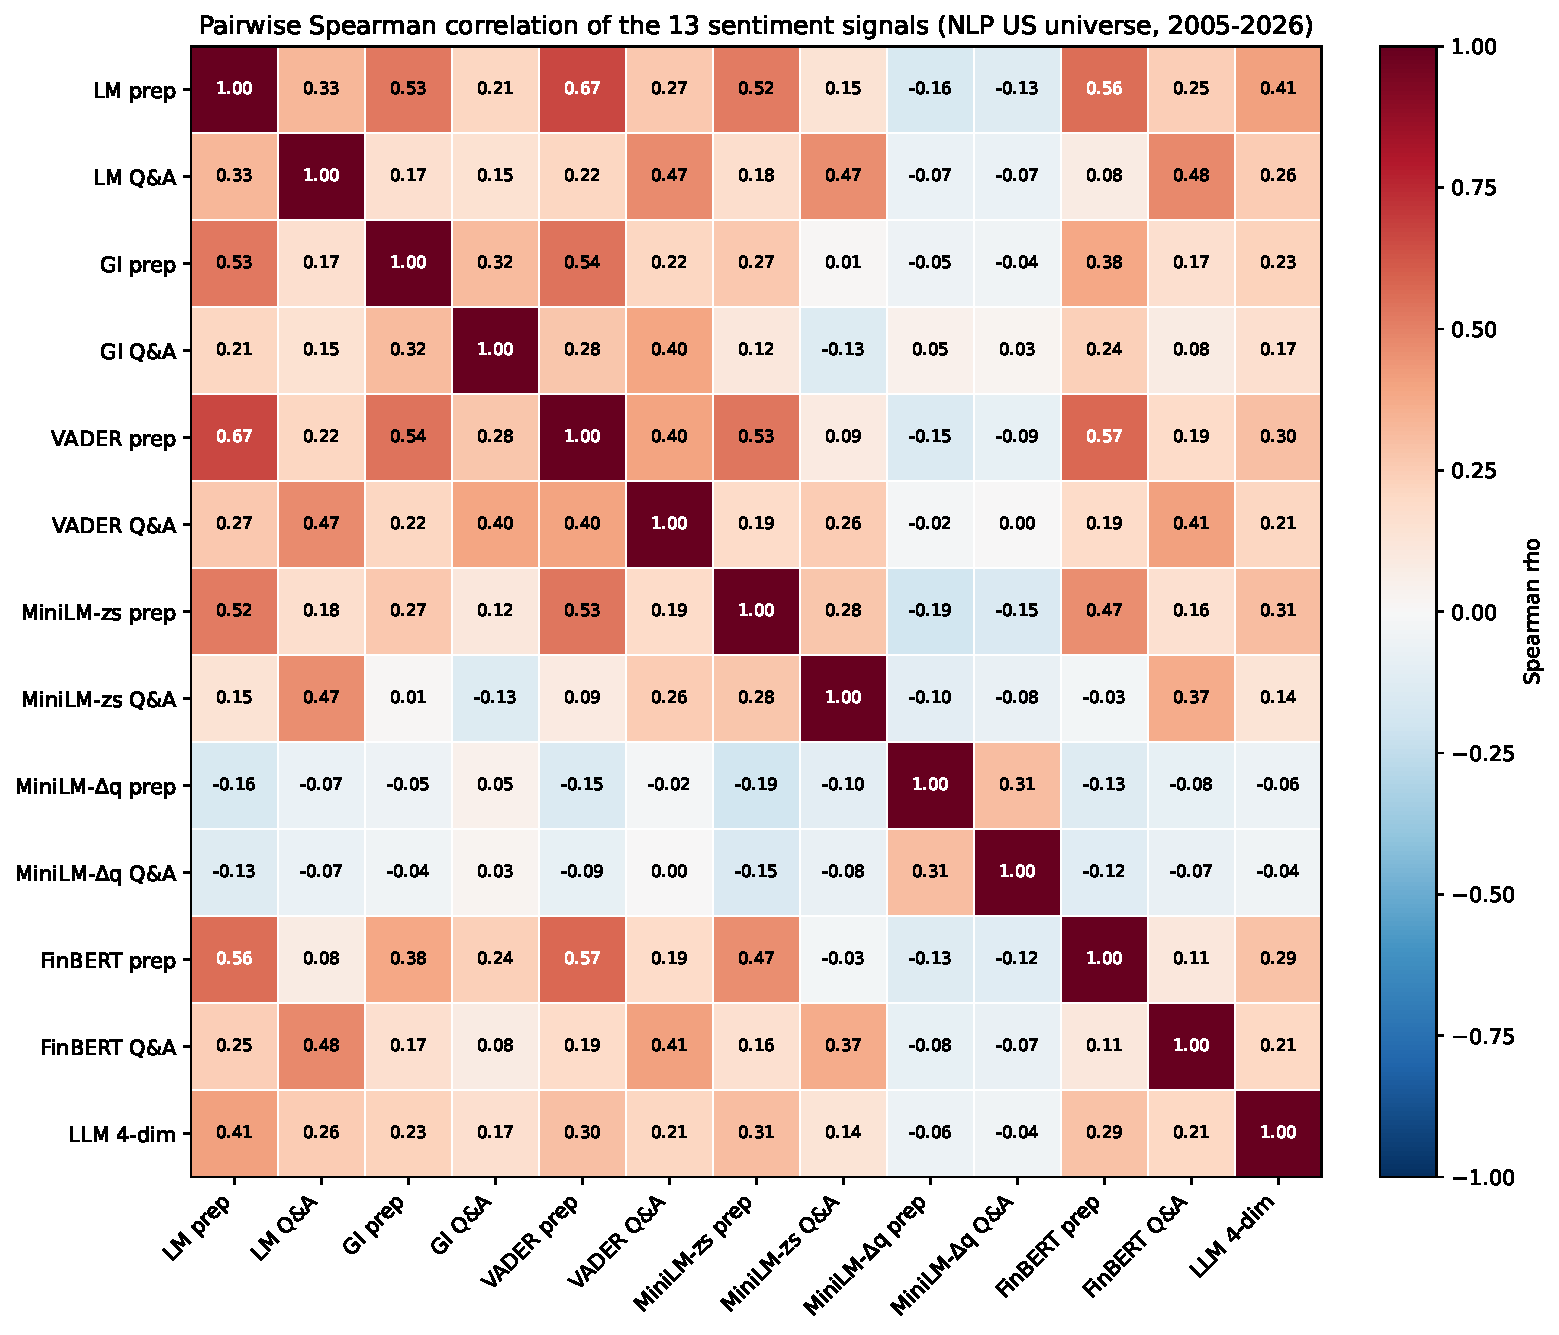
\includegraphics[width=0.7\linewidth]{files/figure_21_1_signal_d-c98aba29058901425df7938318f10c92.pdf}

It clarifies how much each method is a re-skinning of the others. The average off-diagonal correlation is 0.18, low enough that the methods are far from interchangeable on this sample. Four clusters stand out. The three tone-on-prepared-remarks dictionaries (LM prep, GI prep, VADER prep) cluster together at pairwise correlations of 0.4 to 0.5, with their Q\&A counterparts forming a parallel weaker cluster. FinBERT sits closer to the dictionaries than to the MiniLM family, consistent with the fact that it is a finance-domain fine-tune of a transformer trained to predict the same per-sentence sentiment categories (positive / neutral / negative) that the dictionaries operationalise. The two MiniLM $\Delta$quarter signals are near-orthogonal to every level-based signal, the expected signature of a textual-change construction that measures \textit{what moved} rather than \textit{what tone was struck}. The LLM 4-dim composite is largely orthogonal to every classical method, with pairwise correlations below 0.2 across the board, indicating that the four-axis decomposition (managerial confidence, specificity, surprise-negative, macro-vs-firm risk framing) is articulating dimensions that the single-scalar tone metrics simply do not see. The complementary correlations of each sentiment signal against the Fama-French / Carhart factor returns are reported in TABLE 21.2.

\paragraph{Spanning regression against Fama-French plus momentum}

A high information coefficient establishes that a signal carries cross-sectional information; it does not establish that the information is new. A sentiment score adds nothing to a portfolio already tilted on value, momentum, or quality if it merely re-expresses those exposures, so the question that decides whether a signal is worth trading is whether it earns a return the canonical equity-factor stack cannot explain. The standard tool for answering it is the \textit{spanning regression}, which regresses the signal's long-short portfolio return on the factor stack and reads the intercept as the part of that return the factors leave unexplained; we report it for every sentiment method in TABLE 21.2.

\textbf{TABLE 21.2: Spanning regressions of sentiment long-short portfolios on the Fama-French five-factor model augmented with Carhart momentum (US data, monthly, 2006-2026).} Following the convention of \cite{tetlock2007giving}, \cite{loughran2011liability}, and \cite{ke2019predicting}, we test whether each sentiment signal carries information \textit{net of} the canonical equity-factor stack by regressing its long-short portfolio return on the Fama-French five factors plus momentum. The construction is the standard \textit{monthly-rebalanced} one. At each month-end we forward-fill each stock's most recent earnings-call sentiment score (with a three-month stale-out, matching the natural quarterly call cadence), decile-sort the cross-section of stocks with a non-stale score, and form an equal-weighted long-short portfolio (top decile minus bottom decile). The realised one-month-forward return of each stock is taken from \texttt{mlfi\_us\_data} (column \texttt{R1M\_Usd}, the same monthly-return column used throughout the book). The cross-section requires at least 30 stocks to enter the sort. The resulting series is a non-overlapping monthly long-short return; spanning the 2006-2026 window yields 236 to 240 monthly observations per method. The factor returns (MKT-RF, SMB, HML, RMW, CMA, MOM) are pulled from Kenneth French's data library, the same source used in Chapter 3, with Newey-West HAC standard errors at five lags. The intercept (\texttt{Alpha}, annualised, in percent) tests whether the sentiment portfolio earns return unexplained by the six factors; the \texttt{R\textsuperscript{2}} measures how much of the sentiment-portfolio variance is \textit{explained} by FF6 (low R\textsuperscript{2} = orthogonal signal). Significance of the alpha intercept and of each factor loading, read from Newey-West t-statistics, is flagged with stars: * denotes p \textless  0.10, ** p \textless  0.05, *** p \textless  0.01.

\bigskip\noindent
\begin{tabular}{p{\dimexpr 0.091\linewidth-2\tabcolsep}p{\dimexpr 0.091\linewidth-2\tabcolsep}p{\dimexpr 0.091\linewidth-2\tabcolsep}p{\dimexpr 0.091\linewidth-2\tabcolsep}p{\dimexpr 0.091\linewidth-2\tabcolsep}p{\dimexpr 0.091\linewidth-2\tabcolsep}p{\dimexpr 0.091\linewidth-2\tabcolsep}p{\dimexpr 0.091\linewidth-2\tabcolsep}p{\dimexpr 0.091\linewidth-2\tabcolsep}p{\dimexpr 0.091\linewidth-2\tabcolsep}p{\dimexpr 0.091\linewidth-2\tabcolsep}}
\toprule
Method & n & Alpha (\%/yr) & t (NW) & R\textsuperscript{2} & $\beta$ MKT-RF & $\beta$ SMB & $\beta$ HML & $\beta$ RMW & $\beta$ CMA & $\beta$ MOM \\
\hline
Loughran-McDonald (prep, mgmt) & 240 & -1.9 & -0.61 & 0.012 & 0.08 & 0.00 & 0.00 & 0.07 & -0.11 & 0.02 \\
Loughran-McDonald (Q\&A, analysts) & 240 & -2.5 & -1.16 & 0.017 & 0.05 & -0.05 & -0.03 & 0.10 & 0.03 & 0.05 \\
Harvard GI (prep, mgmt) & 240 & -0.4 & -0.17 & 0.019 & 0.07 & -0.08 & -0.07 & -0.02 & 0.07 & -0.04 \\
Harvard GI (Q\&A, analysts) & 240 & +0.6 & +0.29 & 0.033 & -0.03 & 0.02 & -0.09 & -0.01 & -0.06 & 0.03 \\
VADER (prep, mgmt) & 240 & -3.5 & -1.47 & 0.029 & 0.08** & -0.00 & 0.06 & 0.02 & -0.13 & 0.00 \\
VADER (Q\&A, analysts) & 240 & -0.2 & -0.09 & 0.035 & -0.02 & -0.05 & -0.08 & 0.07 & -0.00 & 0.03 \\
MiniLM max-seed (prep, mgmt) & 240 & -4.4 & -1.64 & 0.111 & 0.17*** & -0.11 & 0.24** & -0.19* & -0.16 & 0.09** \\
MiniLM max-seed (Q\&A, analysts) & 240 & -4.3** & -2.14 & 0.037 & 0.06 & -0.04 & 0.16** & -0.07 & -0.08 & 0.08* \\
MiniLM $\Delta$quarter (prep, mgmt) & 237 & -1.6 & -0.76 & 0.046 & 0.03 & -0.18** & 0.15* & -0.02 & -0.22** & 0.02 \\
MiniLM $\Delta$quarter (Q\&A, analysts) & 236 & +0.7 & +0.41 & 0.007 & -0.02 & -0.06 & 0.01 & -0.06 & -0.04 & 0.00 \\
FinBERT (prep, mgmt) & 240 & -0.8 & -0.34 & 0.046 & 0.09** & -0.16* & 0.14 & -0.14 & -0.11 & -0.01 \\
FinBERT (Q\&A, analysts) & 240 & -0.6 & -0.39 & 0.028 & 0.06 & -0.11 & 0.08 & -0.12 & -0.04 & 0.05 \\
LLM 4-dim composite (Llama-3.1-8B) & 240 & +6.0* & +1.70 & 0.011 & 0.04 & -0.09 & 0.13 & -0.11 & -0.09 & 0.05 \\
\bottomrule
\end{tabular}

\bigskip

Three observations land cleanly on this table. First, the R\textsuperscript{2} values are uniformly small (between 0.01 and 0.11), which is the central methodological finding: every sentiment long-short portfolio in this table is largely \textit{orthogonal} to the six Fama-French / Carhart factors. The supplementary correlation matrix (computed alongside the table) confirms this: the largest pairwise correlation between any sentiment portfolio and any factor is 0.25 (MiniLM max-seed prep vs MKT-RF), with the bulk in the 0.00 to 0.15 range. Sentiment is not a hidden re-skinning of momentum or quality on this sample, and the one method that loads materially on the market and the value factors, MiniLM max-seed (prep), is also the method with the largest R\textsuperscript{2} (0.11) and therefore the most explained-away alpha. Second, no method clears the conventional 5\% alpha-significance threshold over this 20-year monthly panel. The closest are MiniLM max-seed (Q\&A) at -4.3\% per year (NW-t -2.14, just over the threshold but the wrong sign) and the LLM 4-dim composite at +6.0\% per year (NW-t +1.70, just under it). The LM, GI, VADER, MiniLM-$\Delta$quarter, and FinBERT alphas all sit between -3.5\% and +0.7\% with NW-t below 1.6 in absolute value. The upshot is that the strong univariate ICs reported in TABLE 21.1 do not translate into statistically significant portfolio alpha over a 240-month sample once the FF6 factor stack absorbs the systematic component. Third, the negative-sign alphas on MiniLM max-seed and VADER are consistent with the negative-IC pattern observed for the same methods in TABLE 21.1: the realised top-decile-minus-bottom-decile portfolio is sign-reversed and would be profitable as a contrarian bet, but neither the univariate IC nor the FF6 alpha is large enough to recommend it as a deployed strategy. The LLM 4-dim composite is the one entry whose alpha and direction both point the right way, but a marginally-significant +6.0\%/yr on a single 20-year US window is not yet evidence of a robust new factor; the look-ahead-bias caveats discussed in Chapter 23 (Llama-3.1-8B's training corpus overlaps the evaluation window) further temper that reading.

This orthogonality also settles a question the literature raises. \cite{habibah2021investor} find that \textit{aggregate} Baker-Wurgler sentiment drives the size and profitability premia; our firm-level signal does not, because a cross-sectional decile long-short differences out precisely the market-wide component a Baker-Wurgler index is built from. The two are both labelled ``sentiment'' but measure different objects, so a mirror regression of each premium on our signal returns loadings that are statistically zero across the board.

How was that table built? The construction is short enough to walk through in full, and worth doing because the single most common error in event-study NLP hides in one of its steps. The code below builds one method, Loughran-McDonald (prep); the full table is the same loop run over the other signal columns.

\begin{verbatim}
import pandas as pd
ff = pd.read_parquet('famafrench_us_factors.parquet')  # FF5 + MOM, monthly
panel = pd.read_parquet('sentiment_panel.parquet')     # per-call scores, keyed by secid = mlfi id
data_ml = pd.read_parquet('mlfi_us_data.parquet',
                          columns=['id', 'date', 'R1M_Usd'])
data_ml['month_end'] = data_ml['date'].dt.to_period('M').dt.to_timestamp('M')
ret = data_ml.rename(columns={'id': 'secid', 'R1M_Usd': 'R1M'})[['secid', 'month_end', 'R1M']]
\end{verbatim}

The forward-fill step takes each call's sentiment score and broadcasts it onto the \textbf{subsequent} month-ends only, with a three-month stale-out matching the natural quarterly call cadence; a newer call for the same firm supersedes the older one via \texttt{drop\_duplicates(keep='last')}. This is where the most common rookie error in event-study NLP sits, so we comment the look-ahead guard explicitly.

\begin{verbatim}
STALE = 3                                                         # months
calls = panel[['secid', 'date', 'lm_tone_prep_mgmt']].dropna()    # one method shown
calls['call_month'] = calls['date'].dt.to_period('M').dt.to_timestamp('M')
sig = pd.concat([calls.assign(month_end=calls['call_month'] + pd.offsets.MonthEnd(k))
                 for k in range(STALE)])                          # k=0,1,2: same / +1 / +2 mo
sig = (sig.sort_values(['secid', 'month_end', 'call_month'])
          .drop_duplicates(['secid', 'month_end'], keep='last')   # latest call wins
          .rename(columns={'lm_tone_prep_mgmt': 'signal'}))
\end{verbatim}

The portfolio step pairs the signal observed at month-end \textit{M} with the \texttt{R1M\_Usd} realised over the \textbf{following} month (\textit{M}, \textit{M}+1], never the same month. We require at least 30 stocks in the cross-section to enter the sort, dropping months that fall below that threshold rather than running five-stock deciles.

\begin{verbatim}
sig['next_month'] = sig['month_end'] + pd.offsets.MonthEnd(1)
df = sig.merge(ret.rename(columns={'month_end': 'next_month'}),
               on=['secid', 'next_month']).dropna()
ls = []
for m, sub in df.groupby('month_end'):
    if len(sub) < 30:                                             # min cross-section
        continue
    sub['bin'] = pd.qcut(sub['signal'], 10, labels=False, duplicates='drop')
    top = sub.loc[sub['bin'] == sub['bin'].max(), 'R1M'].mean()
    bot = sub.loc[sub['bin'] == 0, 'R1M'].mean()
    ls.append({'month_end': m, 'ls_ret': top - bot})
ls = pd.DataFrame(ls).set_index('month_end')['ls_ret']
\end{verbatim}

The spanning regression uses \texttt{statsmodels.OLS} with Newey-West HAC standard errors at five lags, the conventional choice for monthly portfolio returns since consecutive months' decile compositions overlap substantially.

\begin{verbatim}
import statsmodels.api as sm
joined = ff.join(ls, how='inner').dropna()
X = sm.add_constant(joined[['MKT_RF', 'SMB', 'HML', 'RMW', 'CMA', 'MOM']])
fit = sm.OLS(joined['ls_ret'], X).fit(cov_type='HAC', cov_kwds={'maxlags': 5})

def star(p):                                            # significance flags, as in TABLE 21.2
    return '***' if p < 0.01 else '**' if p < 0.05 else '*' if p < 0.10 else ''

facs = ['MKT_RF', 'SMB', 'HML', 'RMW', 'CMA', 'MOM']
alpha_ann = fit.params['const'] * 12 * 100              # annualised alpha, percent
print(f"n={int(fit.nobs)}  alpha_ann={alpha_ann:+.1f}%{star(fit.pvalues['const'])}  "
      f"t_NW={fit.tvalues['const']:+.2f}  R^2={fit.rsquared:.3f}")
print("  " + "  ".join(f"{f}={fit.params[f]:+.2f}{star(fit.pvalues[f])}" for f in facs))
\end{verbatim}

\begin{verbatim}
n=240  alpha_ann=-1.9%  t_NW=-0.61  R^2=0.012
  MKT_RF=+0.08  SMB=+0.00  HML=+0.00  RMW=+0.07  CMA=-0.11  MOM=+0.02
\end{verbatim}

The printed line reproduces the Loughran-McDonald (prep) row of TABLE 21.2 exactly, significance stars included; this method carries no coefficient significant at the 10\% level, so none are flagged, but pointing the same code at \texttt{embed\_zs\_prep\_mgmt} would reproduce the starred market, value, and momentum loadings of the MiniLM max-seed (prep) row.

\paragraph{Tree-based feature attribution}

The spanning regression of the previous subsection is linear and takes one signal at a time. A more demanding question is how a sentiment feature fares when it competes against the \textit{entire} book of firm characteristics inside a single nonlinear model. This is the machine-learning asset-pricing programme of \cite{gu2018empirical}, \cite{freyberger2020dissecting}, and \cite{nagel2021machine}: pool every predictor a quant would realistically use, let a gradient-boosted tree learn the nonlinear cross-sectional map to forward returns, and read off which inputs the fitted model actually relies on. We run that horse race with the earnings-call sentiment scores added to the book's own characteristic set.

We assemble a quarterly \textit{bundle}: the 122 numerical characteristics of the book's US panel, of the kind catalogued by \cite{chen2021open}, joined to the 32 sentiment scores of the companion dataset. The 32 scores are the nine per-bucket sentiment methods of TABLE 21.1 taken over the three speech buckets, together with five structural counts; the companion \texttt{sentiment\_panel.parquet} also carries auxiliary columns (forward returns, regime tags, model rationales) that we exclude from the feature set; the file is already keyed to the book's numerical \texttt{id}. The join is the look-ahead-safe forward-fill of the earlier subsections; each call's scores attach only to quarter-ends on or after the call date, within a two-quarter stale-out.

\begin{verbatim}
import pandas as pd
dml = pd.read_parquet('mlfi_us_data.parquet')                       # 122 numerical characteristics
labels = ['R1M_Usd', 'R3M_Usd', 'R6M_Usd', 'R12M_Usd']
classic = [c for c in dml.columns if c not in ['id', 'date'] + labels]
q = dml[dml['date'].dt.month.isin([3, 6, 9, 12])].copy()           # quarter-end rows only
q['date'] = q['date'].astype('datetime64[ns]')

panel = pd.read_parquet('sentiment_panel.parquet')                 # per-call earnings scores, with id
buckets = ['prep_mgmt', 'qa_mgmt', 'qa_analyst']                    # 32 canonical sentiment scores:
methods = ['finbert', 'gi_tone', 'lm_tone', 'lm_neg_pct', 'lm_pos_pct',   # nine methods x three
           'lm_unc_pct', 'vader', 'embed_zs', 'embed_dist']              # speech buckets (27) plus
sent = [f'{m}_{b}' for m in methods for b in buckets] + [           # five structural counts (5) = 32
    'fog', 'text_distance', 'n_words', 'n_money', 'n_percent']
panel['date'] = panel['date'].astype('datetime64[ns]')
panel = panel.dropna(subset=['id']).astype({'id': 'int'})[['id', 'date'] + sent]
\end{verbatim}

The forward-fill join then attaches each firm's most recent call to every quarter-end, and the classical and sentiment columns are concatenated into the 154-feature design matrix.

\begin{verbatim}
# latest call on-or-before each quarter-end, within ~2 quarters (look-ahead-safe)
bundle = pd.merge_asof(q.sort_values('date'), panel.sort_values('date'),
                       on='date', by='id', direction='backward',
                       tolerance=pd.Timedelta('185D'))
bundle = bundle.dropna(subset=['R3M_Usd', 'lm_tone_prep_mgmt'])     # need label + sentiment coverage
bundle['year'] = bundle['date'].dt.year
feats = classic + sent                                             # 122 + 32 = 154 features
\end{verbatim}

The target is the cross-sectional percentile rank of the next-quarter return \texttt{R3M\_Usd}. Ranking within each quarter removes the market-wide component, which no stock-level feature can forecast, and points the model at the cross-sectional stock-picking task.

\begin{verbatim}
bundle['y'] = bundle.groupby('date')['R3M_Usd'].rank(pct=True)      # per-quarter percentile target
\end{verbatim}

The validation protocol is a strict expanding window. The first ten years form the initial training set; the model is retrained every calendar year and used to predict only the \textit{following} year out of sample, so no fold sees its own future. Feature importance is computed with SHAP on each year's out-of-sample rows, using the model trained on strictly prior data, and pooled across folds. The booster is deliberately shrunk to survive the low signal-to-noise of quarterly returns: 400 shallow trees at a slow learning rate, with row and column subsampling.

\begin{verbatim}
import xgboost as xgb, shap
params = dict(n_estimators=400, max_depth=4, learning_rate=0.01,   # slow, shallow, regularized
              subsample=0.8, colsample_bytree=0.6, min_child_weight=5,
              reg_lambda=1.0, objective='reg:squarederror', random_state=42)
years = sorted(bundle['year'].unique())
shap_pool, imp_year = [], {}
for y in [t for t in years if t >= years[0] + 10]:                 # >= 10y train, retrain each year
    tr = bundle[bundle.year < y]; te = bundle[bundle.year == y]    # expanding train, next-year OOS
    fit = xgb.XGBRegressor(**params).fit(tr[feats], tr['y'])
    shap_pool.append(shap.TreeExplainer(fit).shap_values(te[feats]))    # SHAP on OOS rows only
    imp_year[y] = pd.Series(fit.feature_importances_, index=feats)      # gain importance this fold
\end{verbatim}

Two diagnostics frame the result before the ranking. Out of sample the model earns a mean cross-sectional information coefficient of 0.010 across the eleven annual folds, weakly positive and positive in seven of the eleven years. In squared-error terms it barely separates from the naive benchmark that predicts the median rank: the pooled out-of-sample MSE bottoms out around 35 trees and drifts back above the benchmark thereafter, the shallow-signal, quick-to-overfit regime typical of return prediction, in which measured predictability is, as \cite{avramov2023machine} document, concentrated in hard-to-arbitrage stocks and fragile to economic restrictions and trading costs. The quarterly cross-section is hard, and the exercise is about \textit{relative} importance, not a tradeable forecast. With that caveat, we report the pooled out-of-sample SHAP ranking of all 154 features in TABLE 21.3.

\textbf{TABLE 21.3: Pooled out-of-sample SHAP feature ranking, all 154 features, 2015-2025.} Mean absolute SHAP value of each feature, computed on the out-of-sample rows of each annual expanding-window fold and pooled across folds. The \texttt{family} column is the ten-way factor-taxonomy assignment used for the family breakdown below. Only the top 15 of 154 features are shown.

\bigskip\noindent
\begin{tabular}{p{\dimexpr 0.250\linewidth-2\tabcolsep}p{\dimexpr 0.250\linewidth-2\tabcolsep}p{\dimexpr 0.250\linewidth-2\tabcolsep}p{\dimexpr 0.250\linewidth-2\tabcolsep}}
\toprule
Rank & Feature & Family & Mean abs SHAP \\
\hline
1 & Book\_Value\_PS & Value & 0.0061 \\
2 & rsi\_14 & Momentum & 0.0056 \\
3 & EPS & Value & 0.0044 \\
4 & macd & Momentum & 0.0039 \\
5 & vol\_22 & Volatility & 0.0023 \\
6 & size\_log & Size & 0.0019 \\
7 & Earnings\_Volatility\_Proxy & Quality & 0.0018 \\
8 & llm\_specificity & Sentiment & 0.0017 \\
9 & GP\_to\_Assets\_Novy\_Marx & Profitability & 0.0016 \\
10 & FCF\_yld & Value & 0.0015 \\
11 & beta\_252d & Volatility & 0.0015 \\
12 & FCF\_to\_TBV & Profitability & 0.0015 \\
13 & EPS\_Growth\_1Y & Growth & 0.0014 \\
14 & rel\_str\_252d & Momentum & 0.0014 \\
15 & embed\_zs\_qa\_analyst & Sentiment & 0.0014 \\
\bottomrule
\end{tabular}

\bigskip

The ranking is clear and sobering. The top of the table is owned by classical value and technical characteristics (book value, RSI, earnings, MACD, short-horizon volatility, size), the families that the characteristics-only work of \cite{freyberger2020dissecting} and \cite{han2024cross} repeatedly ranks on top, and that the explainable-AI study of \cite{goswami2025significance}, run over 166 predictors, leads with as well. The strongest sentiment feature, the LLM-derived \textit{specificity} score, ranks eighth, ahead of most fundamentals but behind the leaders; the zero-shot embedding score on analyst Q\&A follows at fifteenth. Four sentiment features reach the top twenty and nine the top fifty, a genuine presence rather than a rounding error, yet the four-axis LLM composite that would head a small, hand-picked baseline falls to twenty-sixth once it must compete against the full characteristic set. We plot the SHAP beeswarm for the fifteen leading features, pooled across the eleven annual out-of-sample folds (2015-2025), in FIGURE 21.2.

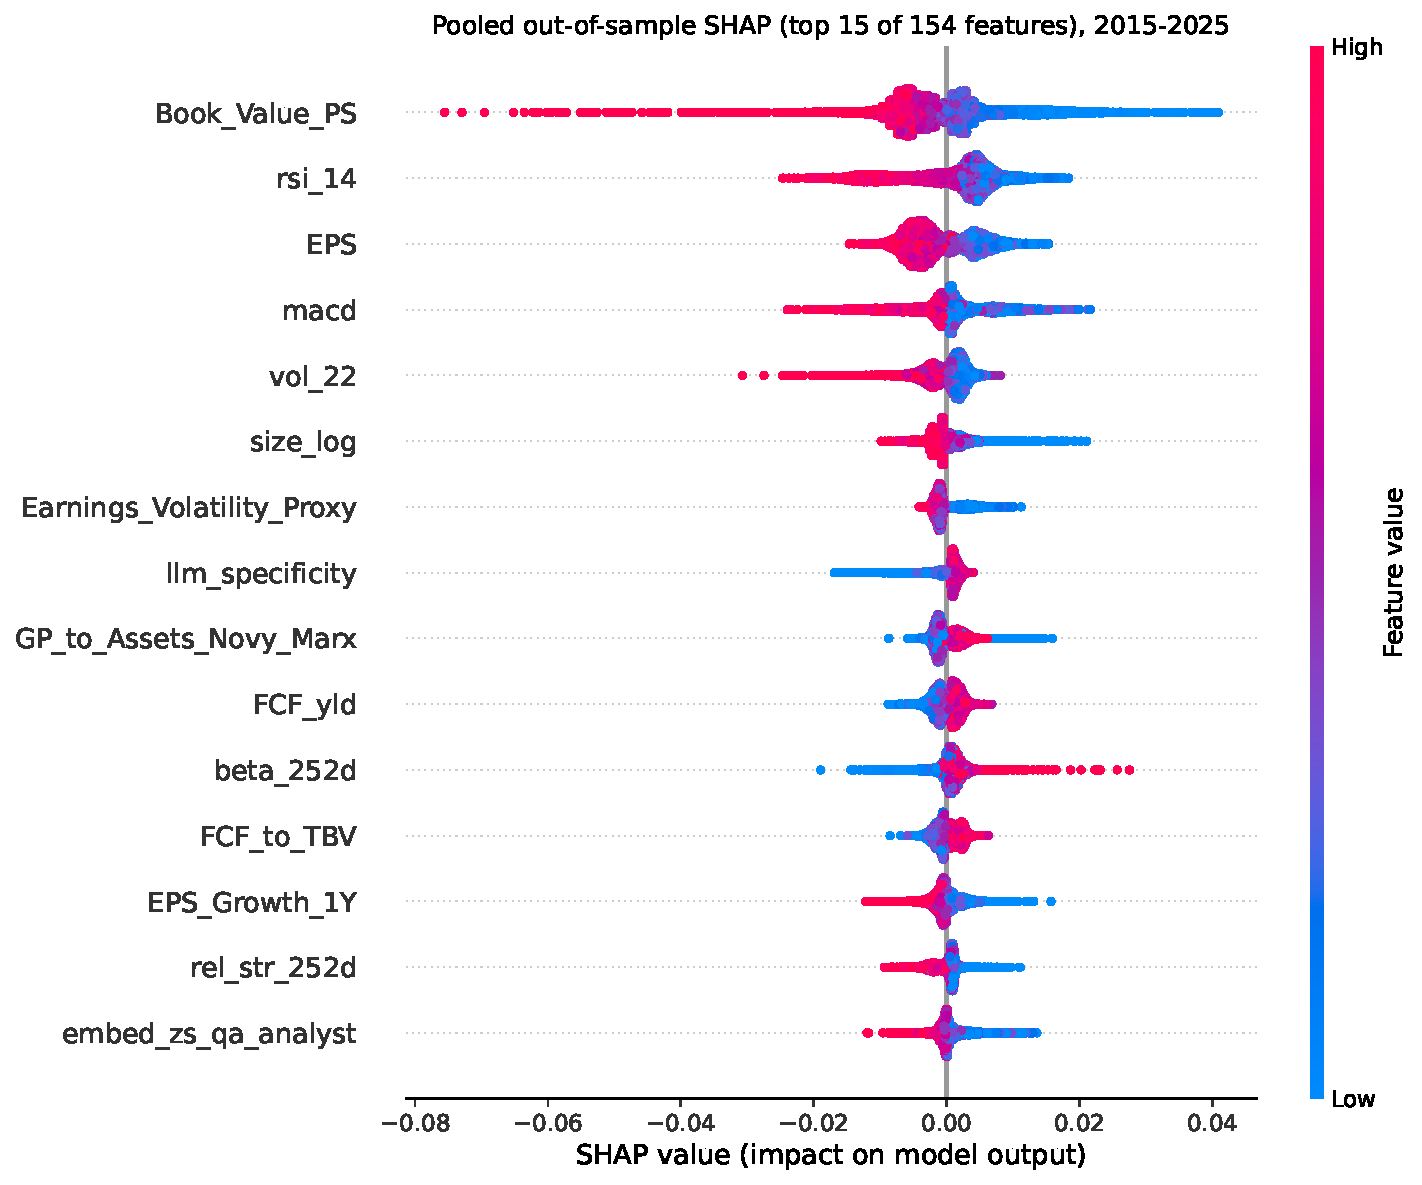
\includegraphics[width=0.7\linewidth]{files/figure_21_2_shap_bee-c4682eafcae615f3a58d916cd47a7d81.pdf}

In FIGURE 21.2 each dot is one out-of-sample firm-quarter, its horizontal position the feature's SHAP contribution to the predicted return rank, and its colour the feature value. The leaders show clean monotone colour gradients; the sentiment features carry diffuse, near-symmetric contributions, the signature of a weak but non-zero signal.

The relative standing of the leading features is broadly stable through time, as the gain-importance paths of FIGURE 21.3 show: the same value, momentum, and volatility characteristics dominate every retrain, their ordering drifting modestly from one year to the next rather than settling into a fixed rank, and the single sentiment feature among the SHAP leaders, LLM specificity, holds a mid-pack line throughout.

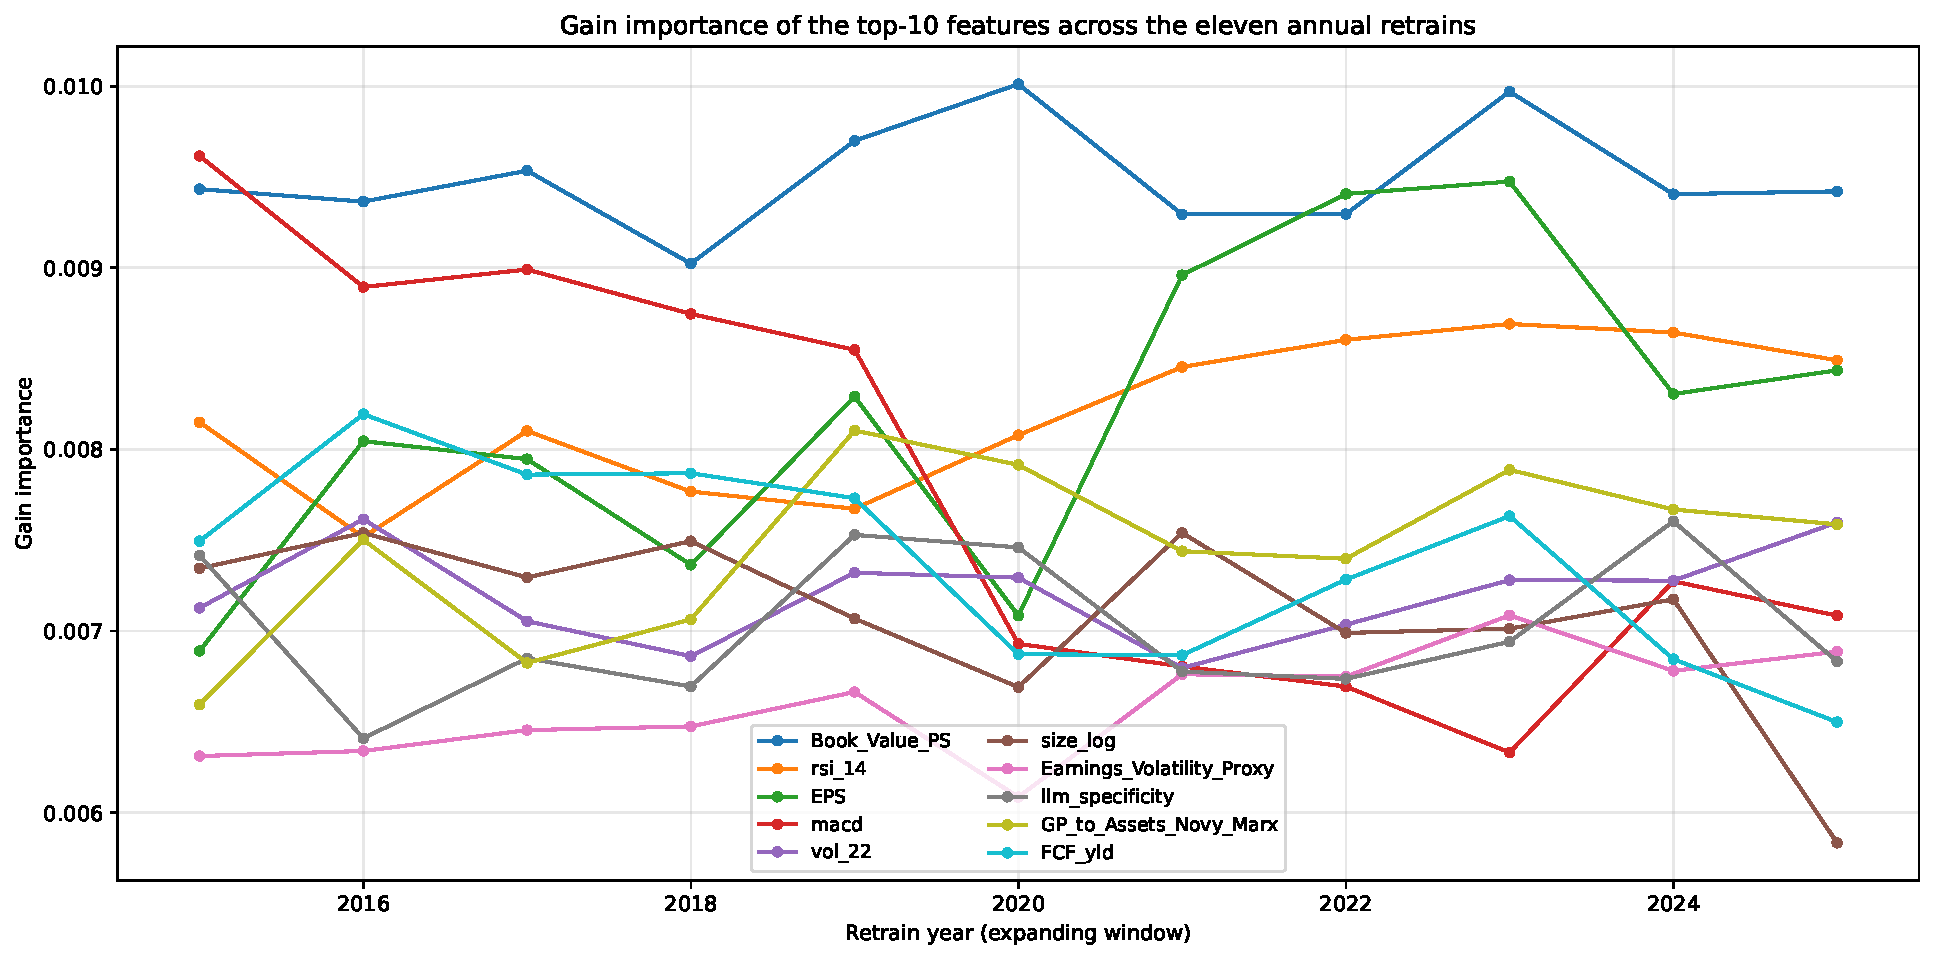
\includegraphics[width=0.7\linewidth]{files/figure_21_3_importan-014d5c1d1f979ba6b51b9e117ad82a23.pdf}

To summarise across all 154 features we group them into ten factor families (value, profitability, quality, growth, investment, momentum, size, volatility, liquidity, and sentiment) and sum the normalised importance within each family for every retrain year, plotting the shares in FIGURE 21.4.

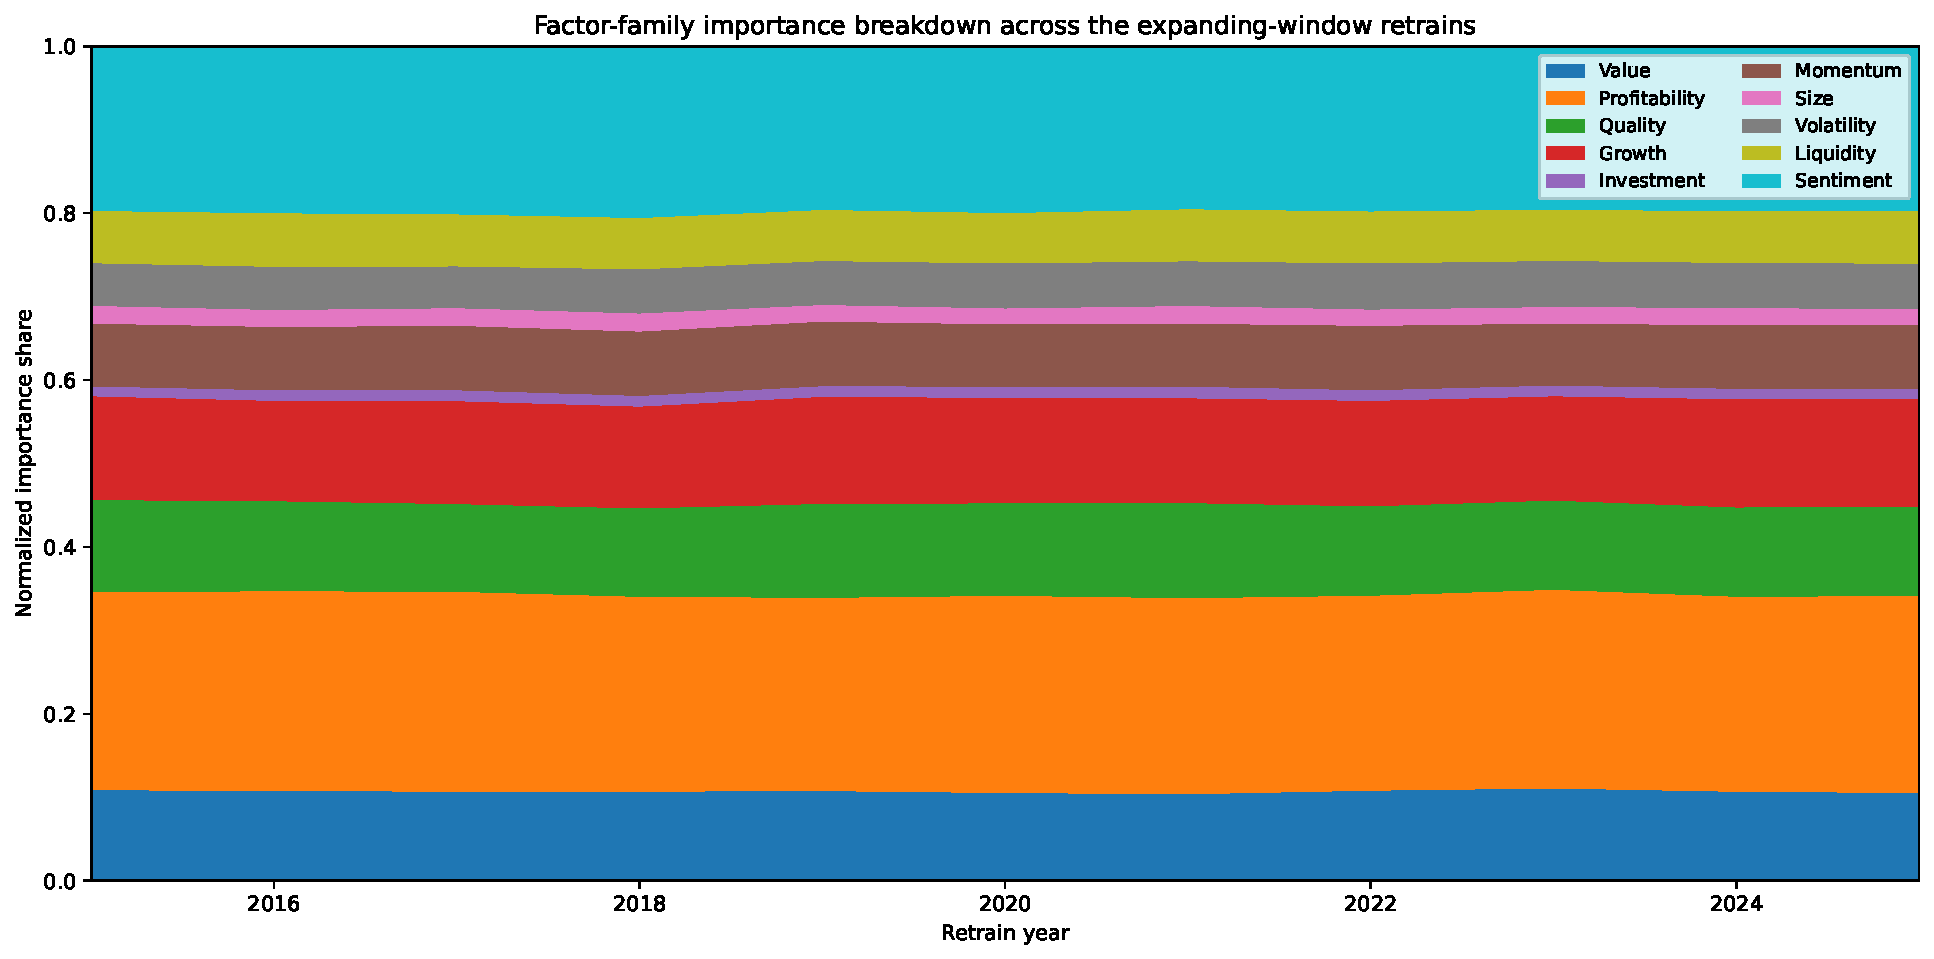
\includegraphics[width=0.7\linewidth]{files/figure_21_4_family_b-fc2726191923f112c5e85240626998b5.pdf}

The family breakdown of FIGURE 21.4 is the headline of this subsection, and it cuts both ways. As a \textit{bloc}, sentiment is the second-largest family the model draws on, taking roughly a fifth of total importance behind only profitability, and its share is steady from 2015 to 2025. But that twenty-percent bloc is almost exactly proportional to headcount, because sentiment supplies 32 of the 154 features. Dividing each family's importance by its number of features, the per-feature contribution is nearly uniform across all ten families, close to ten percent each, with sentiment fractionally at the bottom. The gradient booster, in other words, spreads its reliance evenly: no family, sentiment included, punches above its weight per input. That breadth is literal rather than nominal: the booster picks every one of the thirty-two sentiment scores in at least three of the eleven folds, discarding none of them outright, even though the weakest (the Loughran-McDonald positive-word share on the management Q\&A, which lands 144th of 154) carries a mean absolute SHAP value some fifty times smaller than the leading characteristic. Sentiment earns its collective place through breadth, not through any single dominant score.

The family breakdown treats each feature's importance as a single scalar, and it says nothing about where in the model a score is consulted. To close the subsection we look inside the ensemble itself and extract one of its 400 trees. Below, we plot tree 100, a single full-sample fit that shares the hyperparameters of the expanding-window model of Section 21.7.4, and shade the splits that use a sentiment feature. The result appears in FIGURE 21.5.

\begin{verbatim}
# One tree from the ensemble: a single full-sample fit with the Section 21.7.4
# hyperparameters, used only to look inside the split structure.
import xgboost as xgb
bundle['y'] = bundle.groupby('date')['R3M_Usd'].rank(pct=True)          # per-quarter percentile target
fit_full = xgb.XGBRegressor(**params).fit(bundle[feats], bundle['y'])   # params from Section 21.7.4
tree = fit_full.get_booster().trees_to_dataframe().query('Tree == 100').set_index('ID')
print('root split feature:', tree.loc['100-0', 'Feature'])             # the leading momentum characteristic
\end{verbatim}

\begin{verbatim}
root split feature: rsi_14
\end{verbatim}

With the node table in hand, we assign coordinates, spreading the leaves evenly and centring each interior node above its two children.

\begin{verbatim}
# Lay the tree out: leaves left to right, each interior node centered above its children.
pos, leaves = {}, []
def place(nid, depth):
    node = tree.loc[nid]
    if node.Feature == 'Leaf':
        leaves.append(nid); pos[nid] = (len(leaves) - 1.0, -depth); return pos[nid][0]
    x = (place(node.Yes, depth + 1) + place(node.No, depth + 1)) / 2    # midpoint of the two children
    pos[nid] = (x, -depth); return x
place('100-0', 0)
\end{verbatim}

We then draw the tree, shading the interior nodes that split on a sentiment feature so they stand out from the classical ones.

\begin{verbatim}
# Draw the tree; sentiment splits are shaded to separate them from the classical splits.
import matplotlib.pyplot as plt
from matplotlib.patches import FancyBboxPatch
fmt = lambda s: '~0' if abs(s) < 1e-6 else f'{s:.3g}'                   # tidy near-zero thresholds
fig, ax = plt.subplots(figsize=(15, 7))
for nid, node in tree.iterrows():
    x, y = pos[nid]
    if node.Feature == 'Leaf':
        ax.text(x, y, f'{node.Gain:+.3f}', ha='center', va='center', fontsize=7, color='#445566'); continue
    is_sent = node.Feature in set(sent)                                # sentiment features get shaded, bold boxes
    for child in (node.Yes, node.No):
        ax.plot([x, pos[child][0]], [y - 0.06, pos[child][1] + 0.06], color='#99aaaa', lw=0.8, zorder=1)
    ax.add_patch(FancyBboxPatch((x - 0.9, y - 0.06), 1.8, 0.12, boxstyle='round,pad=0.02', zorder=2,
                 fc='#f4a259' if is_sent else '#dfe7ef', ec='#c26b18' if is_sent else '#9fb0c0',
                 lw=1.4 if is_sent else 0.8))
    ax.text(x, y, f'{node.Feature}\n< {fmt(node.Split)}', ha='center', va='center', zorder=3,
            fontsize=8, fontweight='bold' if is_sent else 'normal')
ax.set_xlim(-1.5, len(leaves)); ax.set_ylim(-4.6, 0.6); ax.axis('off')
plt.tight_layout(); plt.savefig('images/figure_21_5_ensemble_tree.png', dpi=150, bbox_inches='tight')
\end{verbatim}

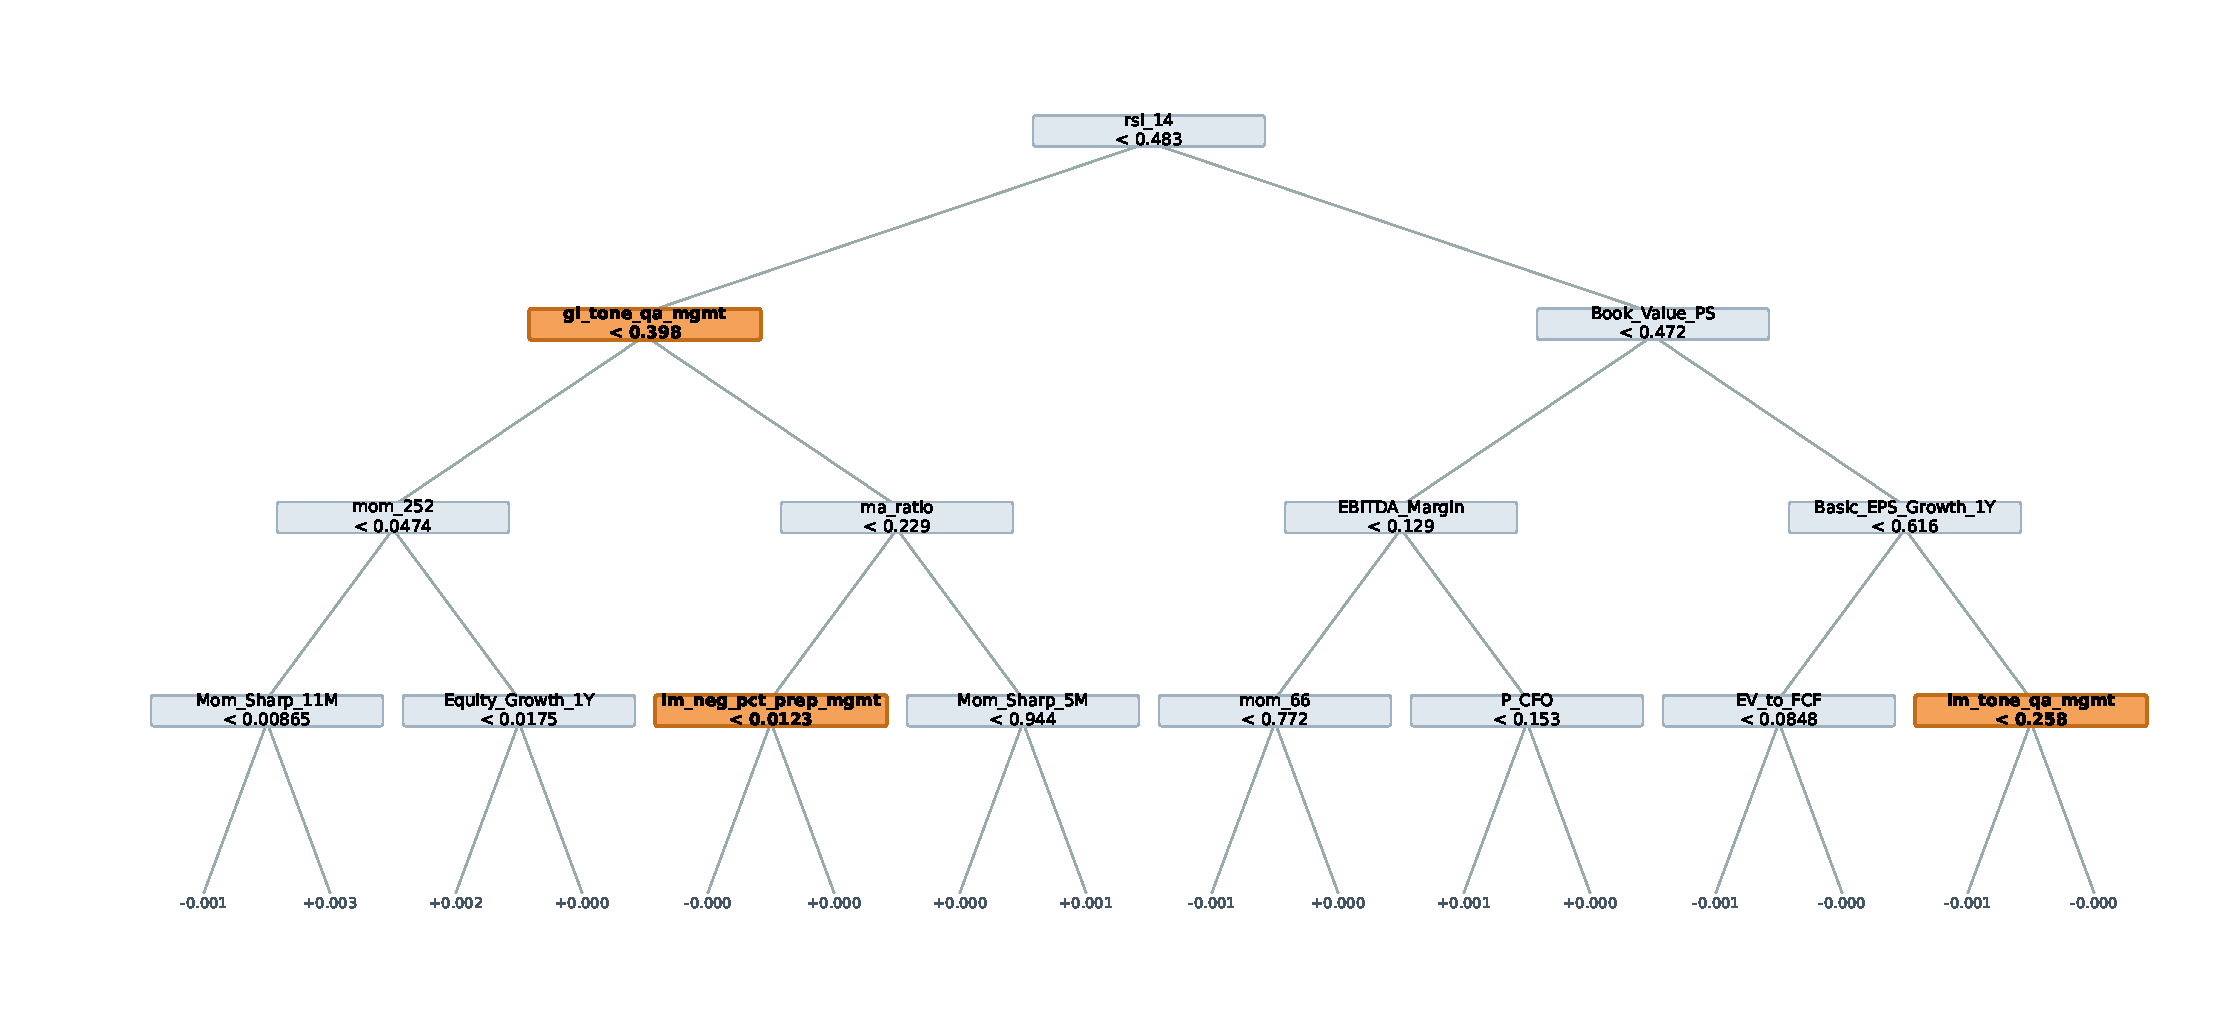
\includegraphics[width=0.7\linewidth]{files/figure_21_5_ensemble-64a8403ad570f013a0e3d710ee52651f.pdf}

The tree of FIGURE 21.5 is revealing. Its root split, the feature the booster consults first for every firm-quarter, is the fourteen-day RSI, a classical momentum characteristic, and the first two levels are dominated by the value, momentum, and volatility characteristics (book value per share, medium-horizon momentum, EBITDA margin) that head the ranking. Sentiment is not shut out of that early geometry, however: a GI-tone score on the management Q\&A splits one level below the root, the LLM-derived specificity score enters at the second level, and a FinBERT prepared-remarks score at the third, three sentiment nodes interleaved with the classical splits rather than relegated to the leaves as residual tie-breakers. We should not over-read a single tree, since it is one of 400 in a learning-rate-0.01 ensemble and its own leaf adjustments are tiny, of the order 0.001 to 0.003 in percentile-rank units, so the aggregate signal remains the weak one documented above. What the tree makes visible is where the sentiment scores enter the model, not that any one of them forecasts returns on its own.

This nonlinear attribution and the linear spanning regression of Section 21.7.3 agree from two directions. The spanning regression found the sentiment portfolios orthogonal to the factor stack, with no reliably significant alpha; the tree finds the individual sentiment features informative but mid-tier, contributing in proportion to their number rather than commanding the model. Neither result places a single text signal above the traditional factors; both cast text-derived features as a genuine, incremental, and unspectacular ingredient. The finding sits between two poles of the literature. At the characteristics-only pole, the linear shrinkage of \cite{kozak2019shrinking} and the nonparametric selection of \cite{freyberger2020dissecting} both recover most cross-sectional predictability from price-trend, liquidity, and volatility characteristics with no text at all. At the text-in-isolation pole, purpose-built text turns first-order when it is the sole input or faces a weak baseline, whether the SESTM learner of \cite{ke2019predicting}, the machine-learning photo-and-text pessimism index of \cite{obaid2022picture}, the priced constraint measure of \cite{buehlmaier2018financial}, or the LLM investment scores of \cite{jha2024chatgpt}. What almost no study reports is the within-model head-to-head we run here, text and the full characteristic panel competing inside one estimator; the textual-factor programme of \cite{cong2019textual} is the closest large-scale precedent, and the manager-sentiment evidence of \cite{jiang2019manager} mirrors our split, with sentiment strong in the aggregate but weaker and conditional in the cross-section.

\paragraph{Sentiment for conditioning factors}

The tree attribution above pools across market conditions. The natural next question is whether sentiment conditions \textit{when} a factor overlay pays off: do the overlays earn their contribution evenly, or only in particular sentiment regimes? The question has a long lineage. A large literature establishes that factor and anomaly premia are not regime-invariant but load on the aggregate sentiment state. \cite{baker2006investor} show that the cross-sectional predictability of hard-to-arbitrage stocks (small, young, volatile, unprofitable, distressed) is itself sentiment-conditional, and \cite{stambaugh2012short} sharpen the point for anomalies: long-short returns are large and significant only following high-sentiment months, and the effect is concentrated in the short leg, where overpricing is hardest to arbitrage away. The same conditioning recurs across the factor zoo, in momentum \citep{antoniou2013cognitive}, in the risk-return tradeoff \citep{yuyuan2011investor}, and in the slope of the security market line \citep{antoniou2016investor}. We therefore characterise the prevailing sentiment regime, shown in FIGURE 21.6, and stratify the Sharpe ratio of each portfolio configuration by it in TABLE 21.4.

Below, we build the regime state variable from the earnings-call panel, the per-quarter cross-sectional mean of the FinBERT sentiment score, and sort the quarters into terciles.

\begin{verbatim}
# The regime state variable: per-quarter cross-sectional mean of the FinBERT
# earnings-call sentiment, sorted into low, medium, and high terciles.
import pandas as pd
sent = pd.read_parquet('sentiment_panel.parquet')
fb = ['finbert_prep_mgmt', 'finbert_qa_mgmt', 'finbert_qa_analyst']     # three call segments
sent = sent[sent['secid'].notna()].copy()
sent['s_mean'] = sent[fb].mean(axis=1, skipna=True)                     # per-call sentiment
sent['quarter'] = sent['date'].dt.to_period('Q').dt.to_timestamp('Q')
s_mkt = sent[sent['quarter'] <= '2026-03-31'].groupby('quarter')['s_mean'].mean()
regime = pd.qcut(s_mkt, 3, labels=['Low', 'Med', 'High'])              # sentiment-regime terciles
\end{verbatim}

We then plot the composite, shading each quarter with a full-height pane in its regime colour.

\begin{verbatim}
# Plot the composite; a full-height background pane colors each quarter by regime.
import matplotlib.pyplot as plt
from matplotlib.patches import Patch
colors = {'Low': '#4c72b0', 'Med': '#b0b0b0', 'High': '#c44e52'}       # cool / grey / warm
q = s_mkt.index
edges = list(q[:-1] + (q[1:] - q[:-1]) / 2)                            # midpoints between quarters
edges = [q[0] - (edges[0] - q[0])] + edges + [q[-1] + (q[-1] - edges[-1])]
fig, ax = plt.subplots(figsize=(11, 4.5))
for i, r in enumerate(regime):
    ax.axvspan(edges[i], edges[i + 1], color=colors[r], alpha=0.16, lw=0, zorder=0)
ax.plot(q, s_mkt.values, color='#333', lw=1.2, marker='o', ms=3.2, zorder=2)
ax.set_xlabel('quarter'); ax.set_ylabel('aggregate sentiment $S_{mkt}$')
ax.legend(handles=[Patch(fc=colors[r], alpha=0.5, label=f'{r} sentiment')
                   for r in ['Low', 'Med', 'High']], ncol=3, frameon=False)
plt.savefig('images/figure_21_6_sentiment_regime.png', dpi=150, bbox_inches='tight')
\end{verbatim}

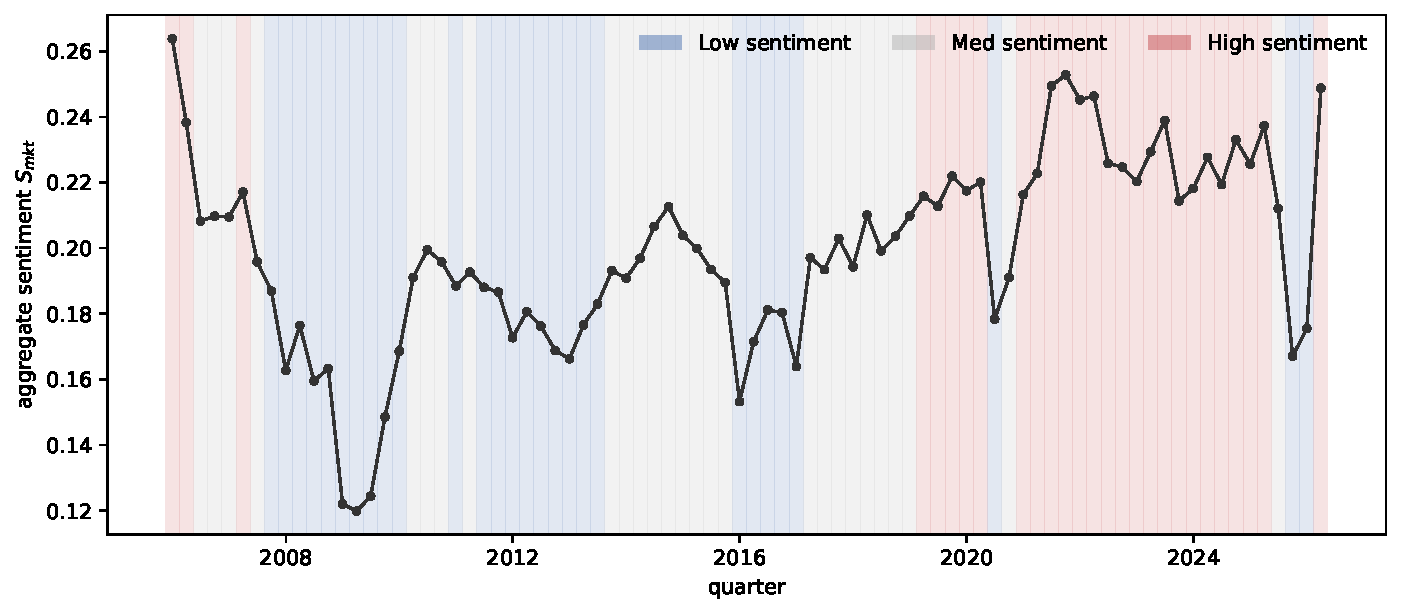
\includegraphics[width=0.7\linewidth]{files/figure_21_6_sentimen-af7a398b47e374892a5e17c6d7756307.pdf}

The regime shown in FIGURE 21.6 is economically legible rather than an artefact of the sorting. The composite sits in its low tercile through the crisis quarters, reaching its sample minimum in the 2008-2009 financial crisis and dipping again in 2016 and during the 2020 pandemic shock, and in its high tercile through the calm expansions of 2006-2007 and 2021-2025. That the tercile of an aggregate earnings-call tone lines up with the familiar risk-on and risk-off phases of the cycle is what lets it serve as a conditioning state rather than noise, and it is this state that TABLE 21.4 stratifies against.

\textbf{TABLE 21.4: Regime-stratified Sharpe ratios, following the sentiment-regime construction of \cite{grobys2021factor}.} Sharpe of each portfolio configuration is reported separately within terciles of an aggregate sentiment composite (low / medium / high) over the same NLP US universe.

\bigskip\noindent
\begin{tabular}{p{\dimexpr 0.250\linewidth-2\tabcolsep}p{\dimexpr 0.250\linewidth-2\tabcolsep}p{\dimexpr 0.250\linewidth-2\tabcolsep}p{\dimexpr 0.250\linewidth-2\tabcolsep}}
\toprule
Configuration & Low & Medium & High \\
\hline
Traditional 6-factor (baseline) & -0.45 & +0.19 & -0.37 \\
+ Loughran-McDonald overlay & -0.40 & +0.05 & -0.97 \\
+ FinBERT prepared overlay & -0.47 & +0.09 & -0.60 \\
+ FinBERT Q\&A overlay & -0.19 & -0.08 & -0.62 \\
+ MiniLM max-seed overlay [baseline] & -0.58 & -0.28 & -0.53 \\
+ MiniLM $\Delta$quarter overlay & -0.38 & +0.06 & -0.55 \\
+ LLM 4-dim overlay (Llama-3.1-8B) & -0.26 & -0.08 & +0.76 \\
+ All-sentiment composite & -0.39 & -0.12 & -0.88 \\
\bottomrule
\end{tabular}

\bigskip

The regime is operationalised as simply as possible: we sort months into terciles of an aggregate sentiment composite and compute the Sharpe of each configuration within each tercile, following the sentiment-conditioning approach that \cite{grobys2021factor} apply to factor momentum. Cleaner state variables are available, among them the partial-least-squares aligned sentiment index of \cite{huang2015investor} and the Markov regime-switching formulation of \cite{chung2012when}, but the tercile split keeps the conditioning transparent and avoids fitting a regime model on the same short sample.

The result cuts against the grain of that literature, and instructively so. The classical overlays, the Loughran-McDonald, FinBERT Q\&A, MiniLM max-seed, and all-sentiment-composite configurations, all collapse in the high-sentiment regime, with Sharpes ranging from -0.53 to -0.97. This is the reverse of what the canon would predict for a genuine mispricing factor: \cite{stambaugh2012short} find anomaly premia are largest, not smallest, following high sentiment, and \cite{grobys2021factor} report that factor momentum is more pronounced when sentiment is high. The most economical reading of our table is that these sentiment overlays are largely contrarian bets whose edge is already priced by the time aggregate sentiment is elevated, so a long-short sort on the signal has little left to harvest. The MiniLM $\Delta$quarter overlay (Lazy Prices on embeddings) is the only embedding configuration to recover a small positive Sharpe (+0.06) in the medium regime, but it too collapses in the high regime (-0.55): the textual-change signal carries genuine information about firm-level dispersion yet does not escape the regime-conditioning that affects every level-based or change-based classical method.

The single exception is the LLM 4-dim overlay, the only configuration with a positive Sharpe in the high-sentiment regime (+0.76 against a baseline of -0.37 and a worst-overlay of -0.97). It is, in other words, the only overlay that behaves the way the classical literature says a genuine mispricing factor should, earning its premium precisely when sentiment-driven overpricing is most acute. We read this as the LLM's four-axis decomposition, managerial confidence net of the macro-vs-firm risk-framing dimension, capturing a textual signal that the classical methods compress into a single sentiment scalar and therefore mistime in exactly the high-sentiment states where it matters most.

Two cautions temper the reading before it hardens into a claim. First, the sample window is finite, and conditional asset-pricing tests are notoriously easy to fool: \cite{novymarx2014predicting} shows that patently spurious conditioning variables, from the weather to sunspots, appear to ``predict'' anomaly performance about as well as economically motivated ones, so a single regime-stratified table is suggestive rather than decisive. Second, the pattern may not travel; \cite{salurekinci2023anomalies} find the sentiment-anomaly link is not universal internationally and is heavily mediated by the size factor. We therefore read TABLE 21.4 as an indicative empirical regularity, consistent with the modern text-sentiment strand that builds the regime bottom-up from language rather than from a slow survey index \citep{garcia2013sentiment, calomiris2019news}, and sufficiently striking to be worth flagging as a research direction rather than as evidence of a robust new factor.

\subsubsection{Coding exercises}

\begin{enumerate}
\item Using the \texttt{gensim} library or a similar implementation, train a Word2Vec
model on a corpus of financial text (e.g., a set of 10-K filings from
SEC EDGAR, or a collection of news headlines from a public dataset).
Examine the resulting embedding space by computing the nearest neighbours
of a handful of financial terms (\texttt{growth}, \texttt{risk}, \texttt{dividend},
\texttt{acquisition}). Do the neighbours match your domain intuition?
\item Download a pre-trained sentence-transformer model (e.g., \texttt{all-MiniLM-L6-v2}
from the \texttt{sentence-transformers} library). Encode the business-description
sections of 50 firm 10-K filings, compute the pairwise cosine-similarity
matrix, and visualise the resulting peer relationships against the firms'
NAICS sector classifications. To what extent does textual similarity track
sector boundaries?
\item Reproduce a reduced-scale version of the feature-importance horse race of
Section 21.7.4. Join the earnings-call sentiment scores in
\texttt{sentiment\_panel.parquet} to a small set of \texttt{mlfi\_us\_data.parquet}
characteristics on a quarterly grid with a look-ahead-safe \texttt{merge\_asof},
train a gradient-boosted tree to predict the per-quarter cross-sectional
percentile rank of the three-month forward return \texttt{R3M\_Usd}, and rank the
features by mean absolute SHAP value. Where does the strongest sentiment
feature land relative to the classical characteristics?
\item Build the aggregate sentiment composite of Section 21.7.5, the per-quarter
cross-sectional mean of the three-segment FinBERT score, and sort the
quarters into low, medium, and high terciles. Form a long-short decile
portfolio on the sentiment signal, report its Sharpe ratio within each
regime, and compare the pattern to the anomaly-after-high-sentiment
prediction of \cite{stambaugh2012short}.
\end{enumerate}

\subsubsection{References}